\documentclass{article}
\usepackage{graphicx} % Required for inserting images
\usepackage{tabularx}
\usepackage{xltabular}
\makeatletter
\providecommand{\ResumeTagging}{}
\providecommand{\SuspendTagging}{}
\makeatother
\usepackage{float}
\usepackage{xcolor}
% --- Fixes for Tab/Input Encoding Issues ---
% \usepackage[T1]{fontenc} 
% \usepackage{textcomp}
\usepackage{minted} 
% ------------------------------------------
% Title definition
\title{

    \begin{center}
        
\includegraphics[width=0.5\textwidth]{images/PolimiLogo.png} 
    \end{center}

    \vspace{1cm}
    
    \Huge\bfseries Best Bike Paths\\
    \vspace{0.5cm}
    
    {\Large Requirement Analysis and Specification Document (RASD)}
}

\author{A. Rubino \and E. Uvinsi \and I. Vinciguerra}
\date{Academic Year 2025/2026}



\begin{document}


\maketitle
\newpage
\tableofcontents
\newpage

%Definition of the outline of the document
\section{INTRODUCTION}
\subsection{Purpose}
The increasing global focus and effort on sustainable mobility and the rising popularity of cycling both as a sport and as a way to navigate around cities have risen new challenges in the everyday life of millions of people. Even if governments are beginning to address the need for new infrastructure for cyclists, the transition is complex and slow and the current infrastructure is often insufficient and outdated. Cyclists often find themselves having to face the danger of unexpected obstacles on their route and of worn-out paths which require maintenance to ensure both safety and navigational efficiency for their daily commutes and training sessions. 
In order to address these needs, a structured and scalable mechanism to systematically collect, consolidate and share data about the conditions of paths becomes necessary. This data has to come from the direct experience of a vast and distributed community of cyclists by offering them a platform that is useful and appealing, regardless of whether they cycle to train or to commute. \\
The purpose of Best Bike Paths (BBP) is to provide a comprehensive software platform that is useful for cyclists as it offers an integrated environment where they can track their session and signal criticalities of paths by therefore contributing to the creation and maintenance of a reliable inventory of bike paths.

\subsubsection{Goals}
\begin{itemize}
    \item G1: Bikers share a path that they have ridden along with other bikers. 
    \item G2: Bikers give other bikers information about the status and the presence of obstacles on paths that they have ridden along. 
    \item G3: Bikers are able to track and record their cycling trips to maintain a log of their activity that contains relevant information about their performance. 
    \item G4: Bikers are presented with a set of paths, comprehensive of information about the path's status and navigational efficiency, between a specified origin and destination. 
\end{itemize}
\newpage

\subsection{Scope}
The core function of the BBP system is to provide a comprehensive, community-driven platform to all types of cyclists. 
The system acts as an intermediary, processing heterogeneous data inputs from various sources, including external providers, and synthesizing this information to generate reliable output for all users. The users who can interact with the platform are: registered users who provide data by tracking their trips and unregistered users who can only browse and search for paths. \\
The system offers its users a dual mode of use which addresses two different kinds of needs: tracking cycling sessions and both adding and accessing directly acquired information about the status of bike paths. The availability of these modes of use depends on the category the user belongs to. \\
The first mode of use is reserved to registered users and it serves as a way to keep a private log of their training sessions and to obtain and store personal performance metrics for each session, together with meteorological information retrieved from external sources, when it is available. \\ The second mode is for both registered and external users and it allows them to access an active inventory of paths which can be visualized on a map and which contain information about their status and their effectiveness. \\ These two modes are completely independent and only have one point of contact: registered users who have tracked a cycling session can decide to publish only the geographical tracking of the path they have ridden along and two types of information about it: an indication of its status and a specification of whether relevant obstacles are present along the way. \\
Data publication by registered users is allowed in only two distinct modes: \textbf{manual mode}, where users manually input the names of the street that compose the path and their status and \textbf{automated mode}, where the system automatically acquires data from the user's mobile device's  GPS, accelerometer and gyroscope to reconstruct the path and to detect significant movements that might be indicative of the presence of obstacles. For both reliability and quality control, when automated mode is used, the user must confirm the elaborated data to make it publishable. \\


\subsubsection{World Phenomena}
\begin{itemize}
    \item WP1: Bikers ride along paths. 
    \item WP2: The bike’s speed changes over time. 
    \item WP3: Bikers track their training sessions with a mobile device that is equipped with the following sensors: GPS, accelerometer and gyroscope. 
    \item WP4: Every path has an origin and a destination. 
    \item WP5: Every path is made of one or more streets. 
    \item WP6: Given the set of streets that compose it, a path is a way of crossing all and only those streets.
    \item WP7: Every path may have obstacles.
    \item WP8: Bikers have a subjective opinion and evaluation of the path’s conditions based on their direct experience.
    \item WP9: Bikers consider each other reliable when it comes to recommending paths.
    \item WP10: GPSs, accelerometers and gyroscopes can perform inaccurate readings.
    \item WP11: The bikers’ coordinates change as they move along a path.
    \item WP12: Meteorological conditions are strictly linked to a specific location and time.
    \item WP13: Bikers actively observe and collect information regarding the path as they travel along it. 
    \item WP14: In the lifetime of a street, new obstacles can appear and old ones can be removed along it.
\end{itemize}


\subsubsection{Shared Phenomena}
\begin{itemize}
    \item SP1: A registered user starts or stops tracking a session on the application.
    \item SP2: Raw sensor data provided by the GPS, accelerometer and gyroscope is actively transmitted and received by the system during the tracking of a session.
    \item SP3: The system can provide all the paths that have been published.
    \item SP4: The system provides the total distance for each published path.
    \item SP5: The system provides performance metrics only to the user who is the owner of the path.
    \item SP6: The system may provide meteorological information only to the user who is the owner of the path.
    \item SP7: The system shows the score for each published path.
    \item SP8: Bikers are provided with a selection of published paths that connect their specified origin and destination, if such published paths exist in the system.
    \item SP9: Users grant the system access to meteorological data from external sources on their device.
    \item SP10: The system allows insertion of publishable paths from the user only in two modes: manual mode and automated mode.
    \item SP11: In manual mode, the user manually inputs the following path data: crossed streets names, status and obstacles, starting point and ending point into the system.
    \item SP12: In automated mode, the user confirms or corrects the information that has been automatically acquired by the system.
    \item SP13: A publishable path is a path that has been manually inserted or automatically registered and then confirmed by the owner of the path.
    \item SP14: The system shows bike paths between an origin and a destination specified by the user ordered by their score, if they exist.
\end{itemize}

\subsection{Definitions, Acronyms, Abbreviations}
\subsubsection{Definitions}
\begin{itemize}
    \item \textbf{Global Positioning System}: a satellite-based navigation system owned by the U.S. government that uses a constellation of orbiting satellites, ground control stations, and receivers to provide precise positioning, navigation, and timing information.
    \item \textbf{Accelerometer}: a sensor that measures linear acceleration (changes in velocity over time) along one or more axes.
    \item \textbf{Gyroscope}: a sensor that measures angular velocity. It detects how fast an object is rotating around a specific axis, which is essential for determining a device's current orientation in space.
    \item \textbf{Meteorological Service Provider}: a formal entity that is responsible for the collection, processing, analysis, forecasting, and dissemination of meteorological and related environmental information and services.
    \item \textbf{Map Service Provider}: a formal entity that provides geospatial infrastructure, data, and rendering capabilities to software applications. It manages the acquisition, storage, and processing of raw Geographic Information Systems (GIS) data such as satellite imagery, vector topology, and traffic signals, allowing client applications to request processed map assets and perform spatial calculations on demand, without maintaining a proprietary geospatial backend.
\end{itemize}

\subsubsection{Acronyms}
\begin{itemize}
    \item \textbf{BBP}: Best Bike Paths
    \item \textbf{GPS}: Global Positioning System
    \item \textbf{GDPR}: General Data Protection Regulation
    \item \textbf{API}: Application Programming Interface
    \item \textbf{OS}: Operating System
\end{itemize}

\subsubsection{Abbreviations}
\begin{itemize}
    \item \textbf{G}: Goal
    \item \textbf{WP}: World Phenomena
    \item \textbf{SP}: Shared Phenomena
    \item \textbf{MSP}: Meteorological Service Provider
    \item \textbf{RU}: Registered User

\end{itemize}


\subsection{Revision History}



\subsection{Reference Documents}
The assignment for this document and all the information included refer to the following
documentation:
\begin{itemize}
    \item The specification for the 2025/26 Requirement Engineering and Design Project for the Software Engineering II course.
    \item The slides on the WeBeep page of the Software Engineering II course.
\end{itemize}


\subsection{Document Structure}
\begin{enumerate}
    \item \textbf{Introduction}: a brief description of the project that follows from the analysis of the specification provided, it highlights the goals of the product and its scope.
    \item \textbf{Overall Description}: a more detailed description of the product that comprehends also real world scenarios and analyses the system from a technical point of view.
    \item \textbf{Specific Requirements}: a detailed list of all the requirements needed in order to satisfy the goals, and their relationship with domain assumptions
    \item \textbf{Formal analysis using Alloy}: a formal description of a portion of real world phenomena analyzed through Alloy in order to highlight inconsistencies between assumptions and phenomena previously modelized.
    \item \textbf{Effort spent}: the time spent by each member of the group to contribute to the realization of this document.
    \item \textbf{References}: reference to documents or tools used for writing this document.
\end{enumerate}
\newpage

\section{OVERALL DESCRIPTION}

\subsection{Product Perspective}
\subsubsection{Scenarios}

\textbf{Registered user tracks a training session in automated mode} \\
Registered user RU wants to track a training session and add it to their personal archive. RU enters the BBP platform with their personal email and password and, once they are logged in, they open the menu and access the "Track new ride" function. The system then asks RU to specify whether they want to use manual or automated mode; RU selects automated mode. At this point, if the system has not been authorized before, it asks RU to grant it access to the mobile device's GPS, accelerometer and gyroscope. Once the system is able to retrieve this data, it signals RU that it is ready to record the session. RU can now start cycling and BBP will take care of elaborating the incoming flow of data to detect when the activity has started and when it is over and to generate an informative record of the session. Once either the system detects that the activity is over or RU signals it is, the system displays an overview of the navigated path and forces RU to confirm or discard status and obstacle information that it has automatically computed before letting RU save the session. Once the user has checked all the information, the record of the activity, enriched with human readable performance metrics and meteorological information (if it is available), is automatically saved and accessible to RU.

\vspace{0.5cm}
\noindent
\textbf{Registered user visualizes a previous training session} \\
Registered User RU wants to visualize a previous training session. RU enters the BBP platform with their personal email and password and, once they are logged in, they open the menu and access the "View my rides" function. The system then visualizes the log of sessions that RU has recorded and allows them to change the visualization order based on the available data (e.g. chronological order, ordered by the length of the sessions etc.). RU finds the session they wanted to visualize and opens it; the system reacts by displaying the path they have ridden along on the map and the associated performance metrics and meteorological data (if present).

\vspace{0.5cm}
\noindent
\textbf{Registered user manually inserts a path} \\
Registered user RU has cycled along a path and wants to upload it on BBP to make it available to other bikers. RU enters the BBP platform with their personal email and password and, once they are logged in, they open the menu and access the "Track new ride" function. The system then asks RU to specify whether they want to use manual or automated mode; RU selects manual mode. The system now allows RU to insert the name of the streets that they have crossed one by one and, at each insertion, it visualizes the street on a map and waits for the user to confirm the address or to correct it. Once RU confirms, the system allows them to select the exact segment of the street that they have ridden along directly on the map and it then shows the result of the selection and waits again for RU's confirmation. Once the street or a segment of it has been correctly selected and confirmed, BBP allows RU to insert information about its status. The reconstruction of the path ends when RU signals they are done. BBP takes care of checking whether the inserted streets actually compose a path and of asking RU to start over with the reconstruction in case they do not. Once the path is validated, RU is shown an overview of it and is given the option to either save the path or discard it. 

\vspace{0.5cm}
\noindent
\textbf{Registered user publishes a path} \\
Registered user RU wants to publish a path to make it available to other users. RU enters the BBP platform with their personal email and password and, once they are logged in, they only have two ways of publishing information: they can either publish an already existent path that is saved on their personal archive or they can create a new one through manual or automated mode and then publish it. In either case, the system will only publish the geographical track of the path, its publication date, RU's username and the status of each street and the obstacles that might appear along it. BBP will also assign it a score that it computes by only using this particular data.

\vspace{0.5cm}
\noindent
\textbf{User visualizes a path}\\
User U wants to find a path that goes from point A to point B. U enters the BBP platform with or without logging in. U then accesses the "Find a path" function from the menu and the system asks them to insert the addresses of their origin and their destination. After each single insertion, BBP visualizes the point on a map and asks U for confirmation or correction. Once both the origin and the destination have been confirmed by U, the system tries to retrieve the existent paths that connect those points. If no suitable path exists, BBP reports an error to U and terminates this workflow; otherwise the system visualizes the best paths, according to their scores, on a map. The number of paths that are shown on the map at the same time is initially set to a default amount that can be modified by U, as far as it does not exceed a fixed upper bound. This upper limit is set by the system in order to achieve a reasonable trade-off between richness and completeness of the information and clearness and neatness of the visualization. U can now select one of the available paths and visualize its details.


\subsubsection{Domain Class Diagrams}
This domain class diagram shows how the entities that are relevant in the domain can be modeled in our system and how the relationships between them could look like. Note that the relationship with the external providers (Map Service Provider and Meteorological Service Provider) and the retrieval of data from the device's sensors (GPS, accelerometer and gyroscope) are not modeled as they are indeed external entities which are simply used as a source of data.

\noindent\makebox[\textwidth][c]{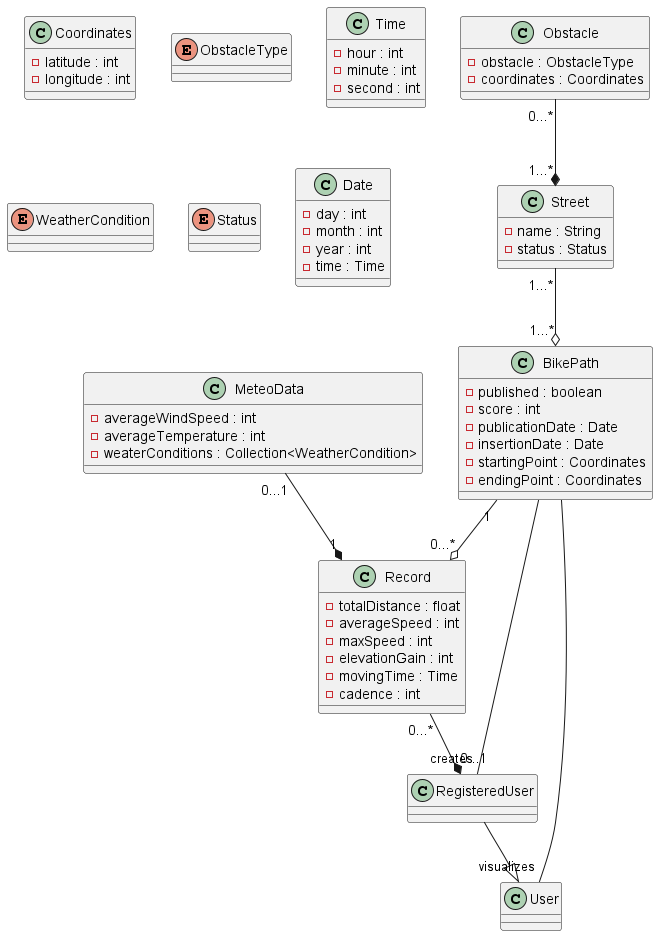
\includegraphics[width=1\textwidth]{images/BBP.png}}


\newpage
\subsubsection{State Diagrams}
The following state machine diagrams have the goal of capturing the behavior of the instances of the main classes that are in the domain class diagram by showing the different status in which they can exist within the system. 

\vspace{0.5cm}
\noindent
\textbf{BikePath lifecycle}\\
This diagram shows the lifecycle of a bike path that can be created in either manual or automated mode. Depending on the mode, the flow is different until the publication status, where the two flows collide again. 

\vspace{0.5cm}
\noindent\makebox[\textwidth][c]{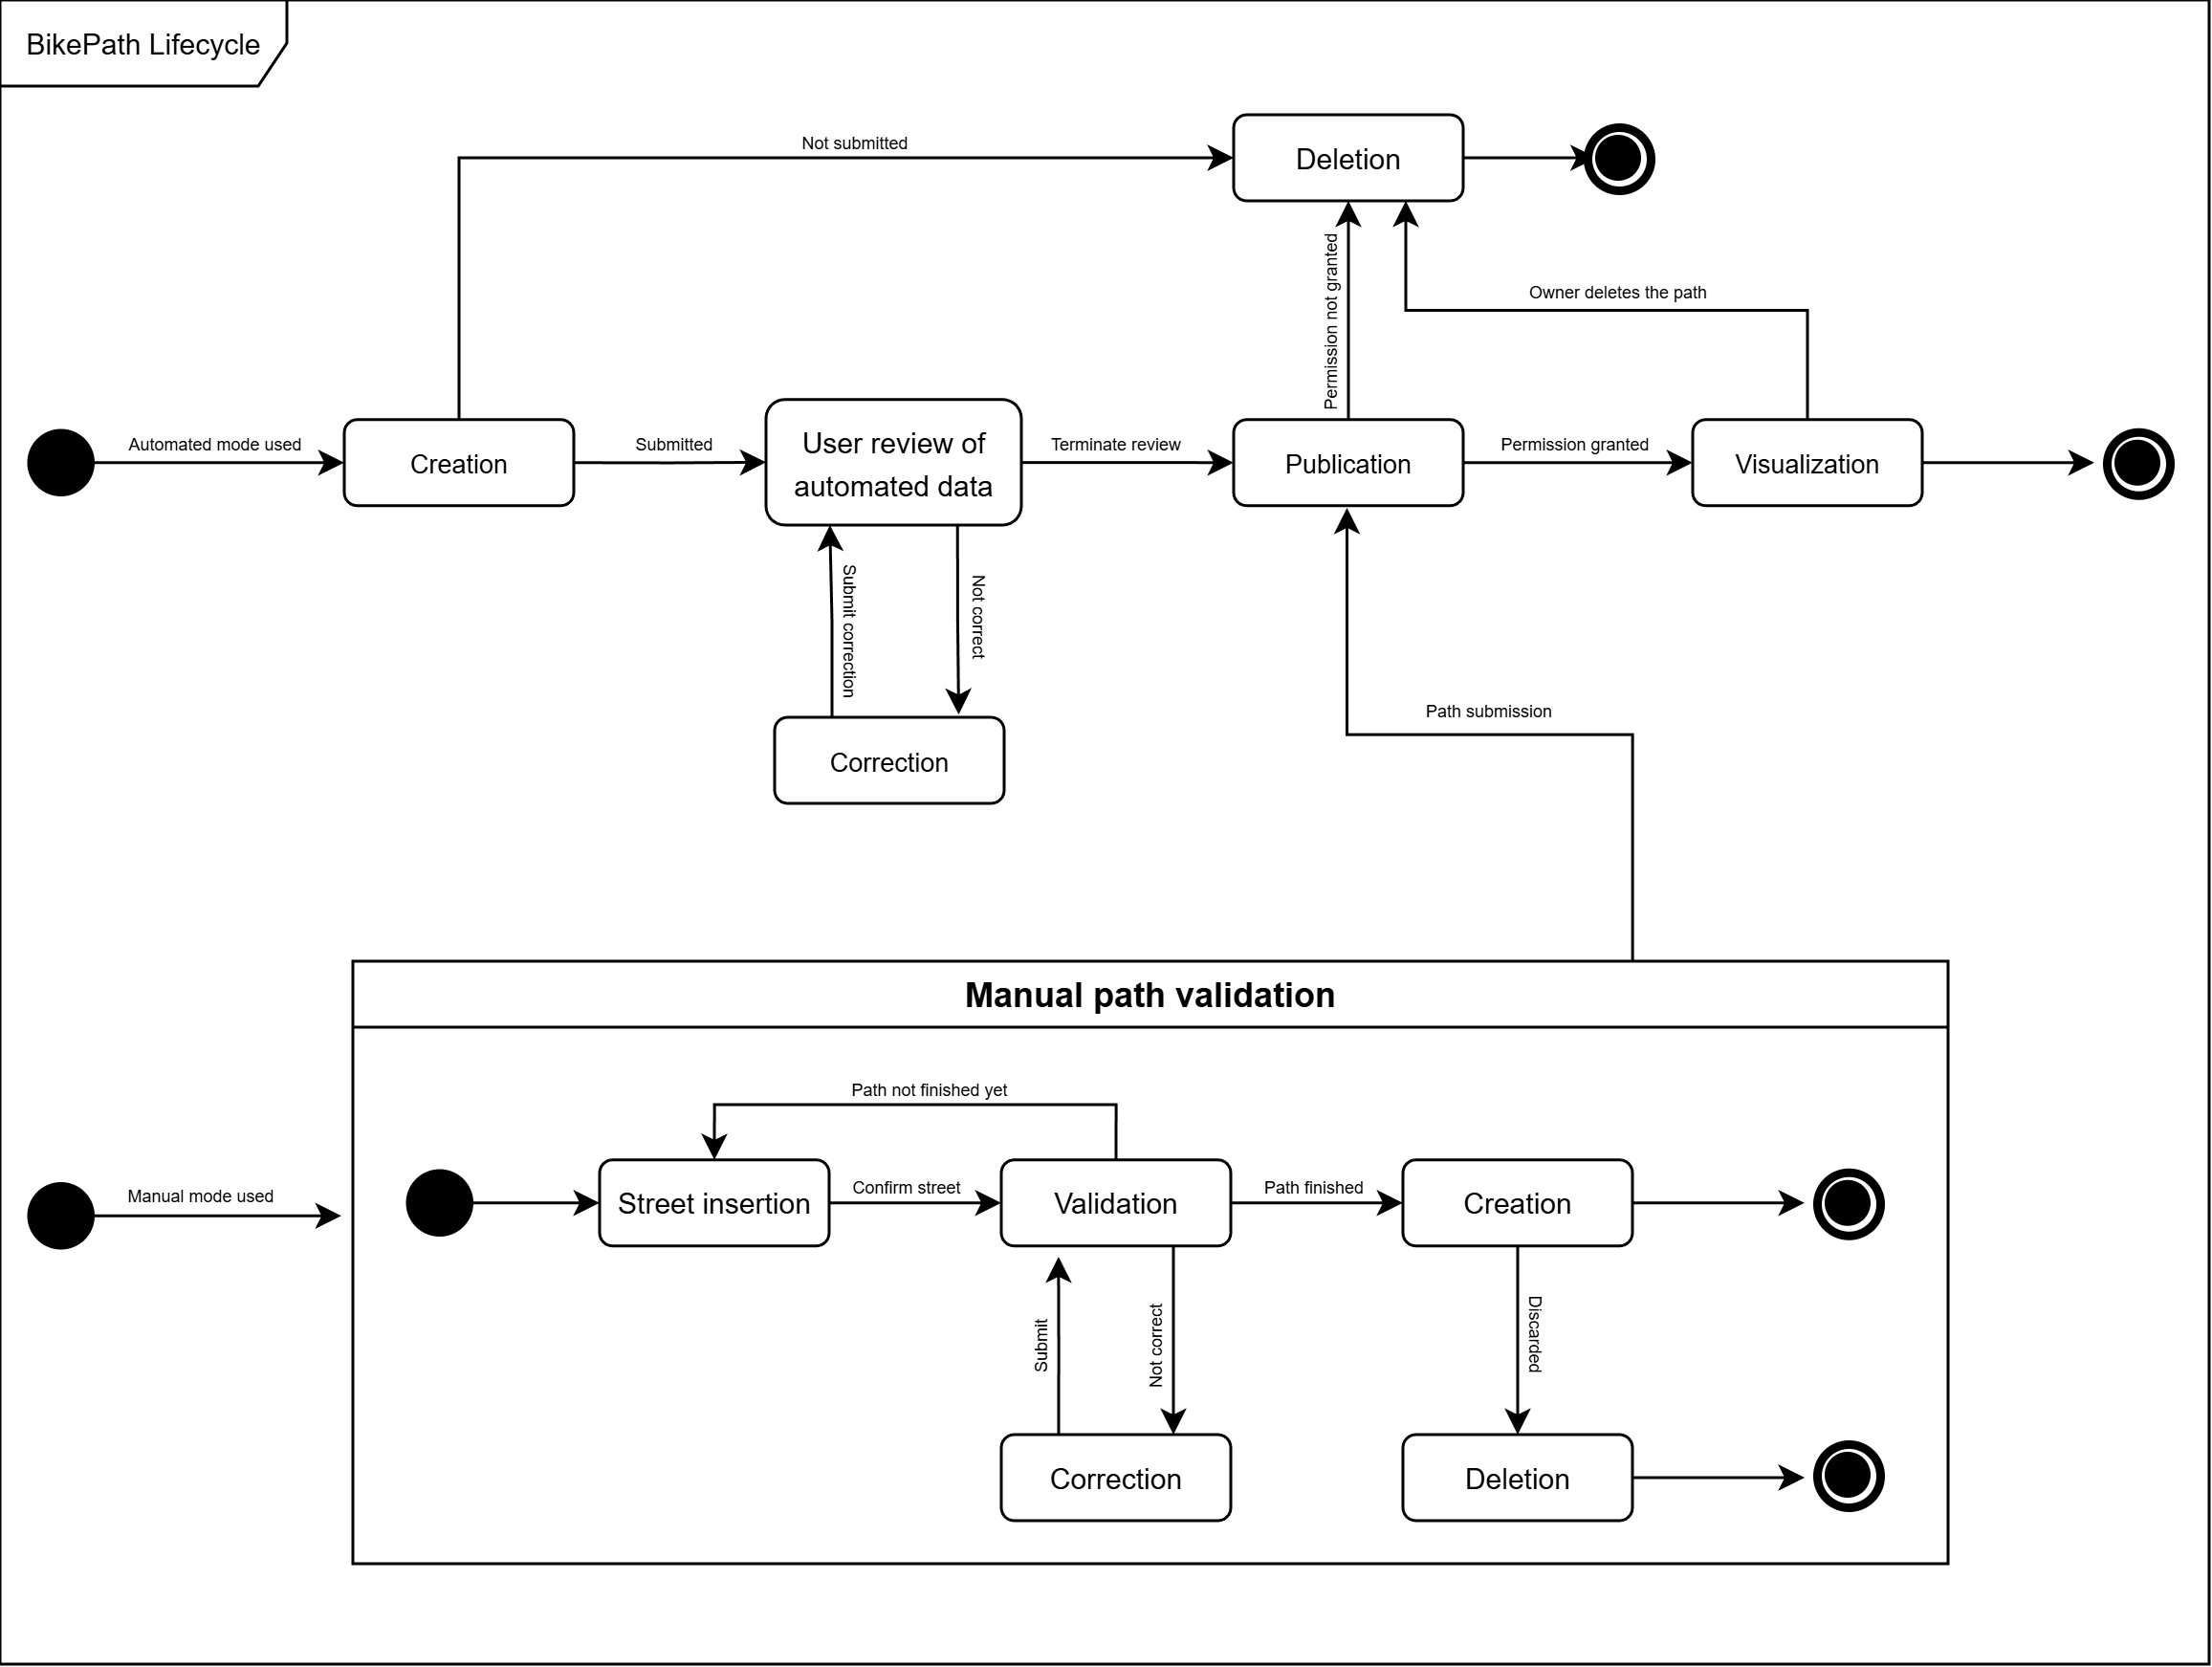
\includegraphics[width=1.5\textwidth]{images/pathLifecycle.png}}

\vspace{1cm}

\noindent
\textbf{Record lifecycle}\\
This diagram shows the lifecycle of a record, which stores the user's performance metrics and can contain meteorological information.

\vspace{2cm}
\noindent\makebox[\textwidth][c]{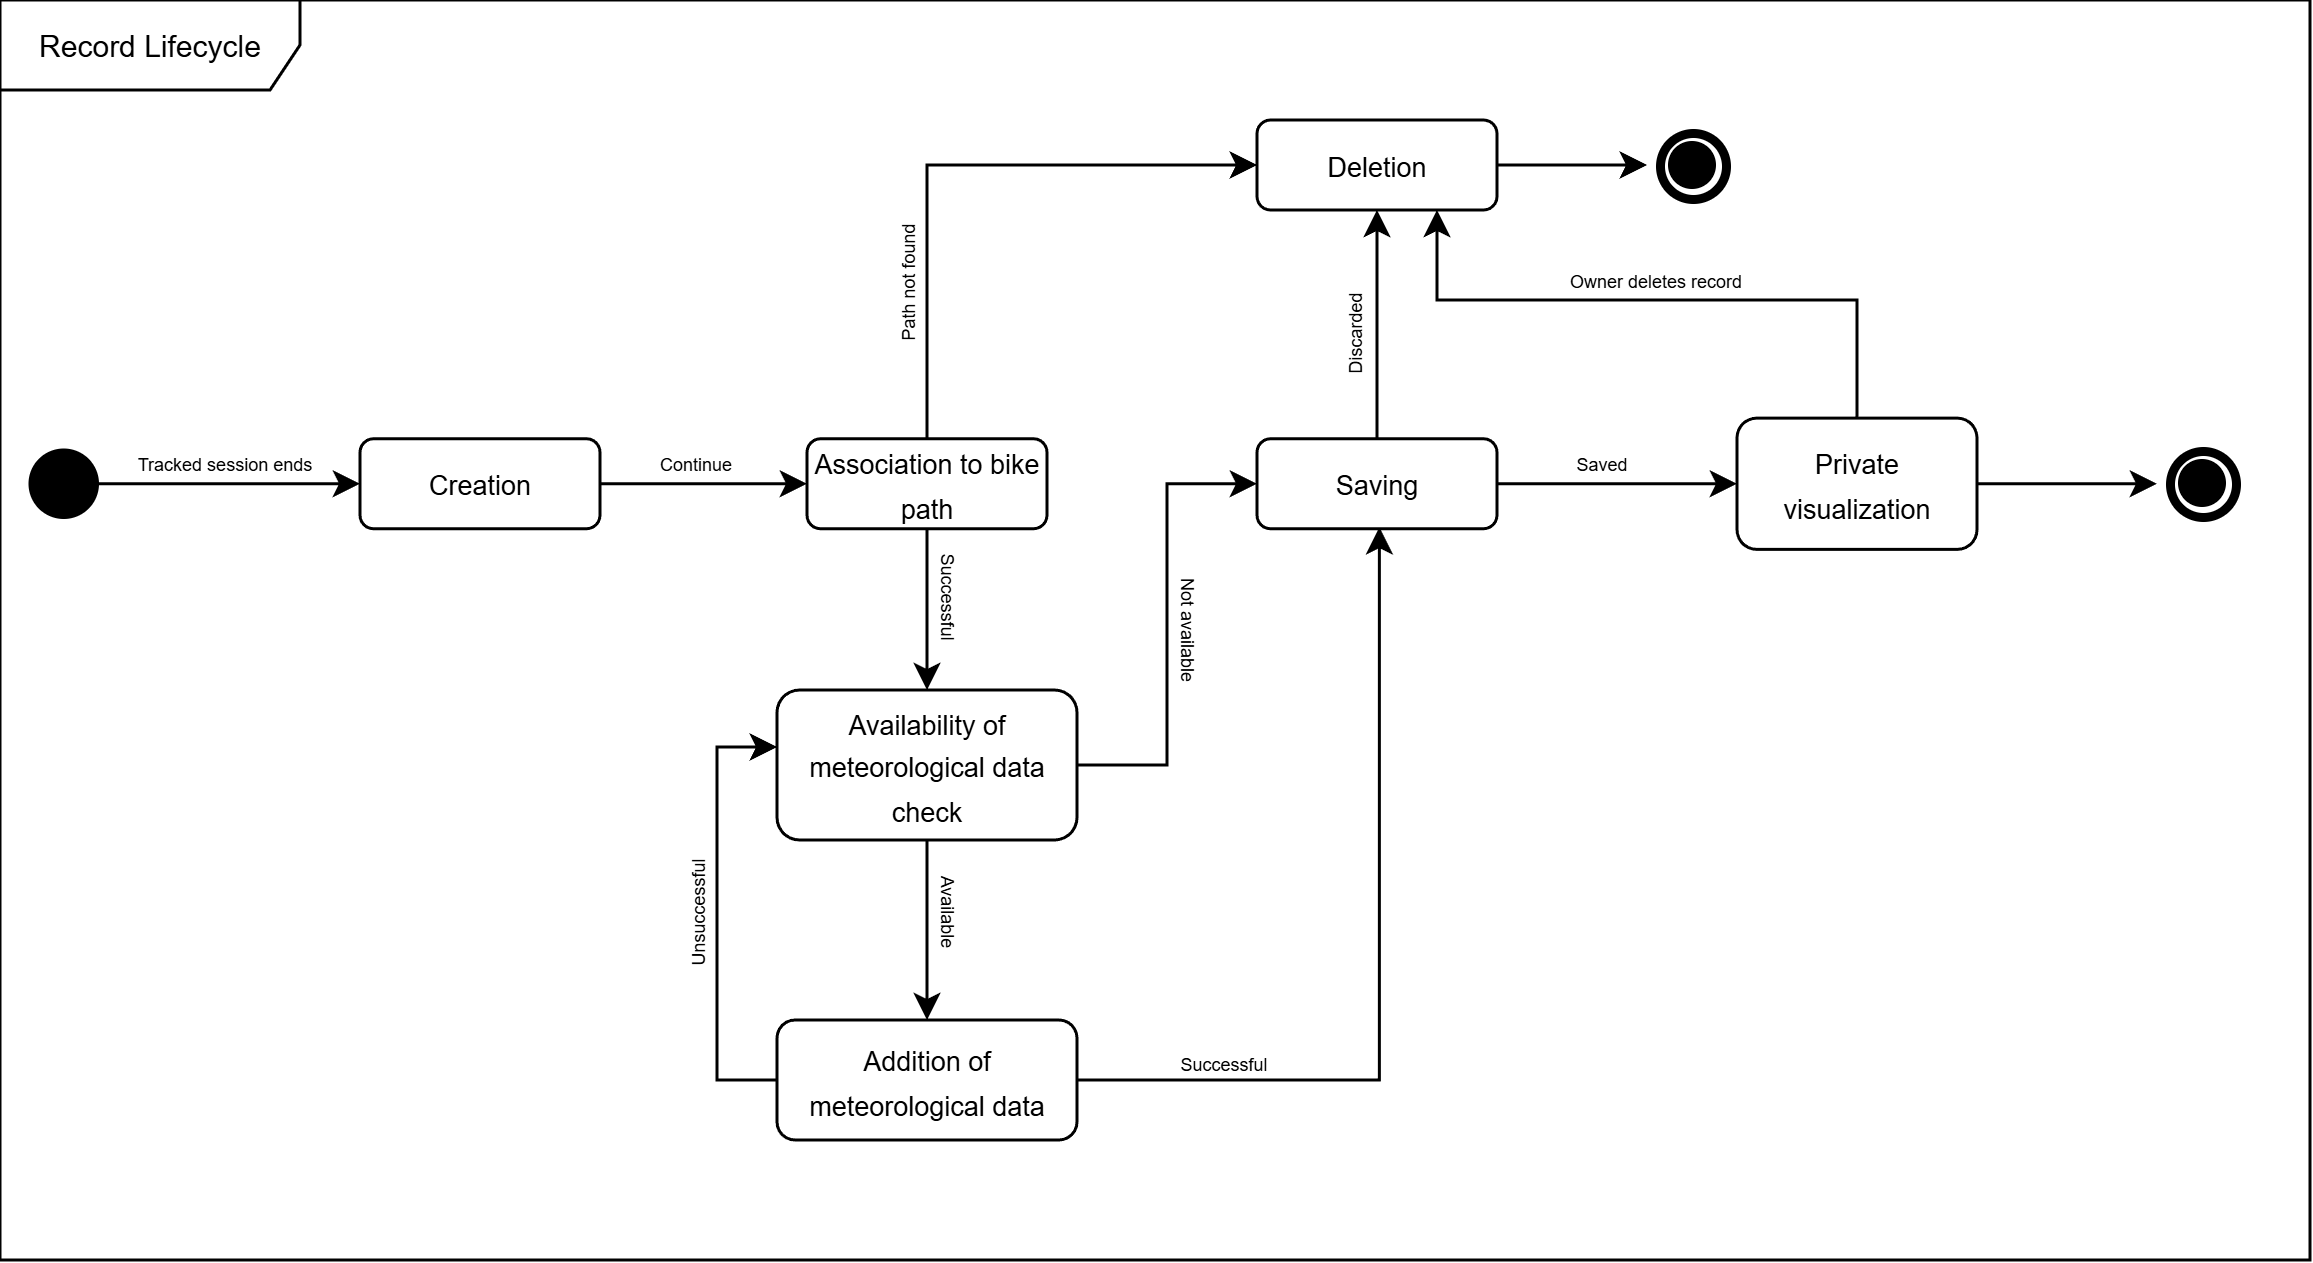
\includegraphics[width=1.5\textwidth]{images/recordLifecycle.png}}

\newpage
\noindent
\textbf{User lifecycle}\\
This diagram shows the lifecycle of both registered and unregistered users when they enter the BBP platform. 

\vspace{2cm}
\noindent\makebox[\textwidth][c]{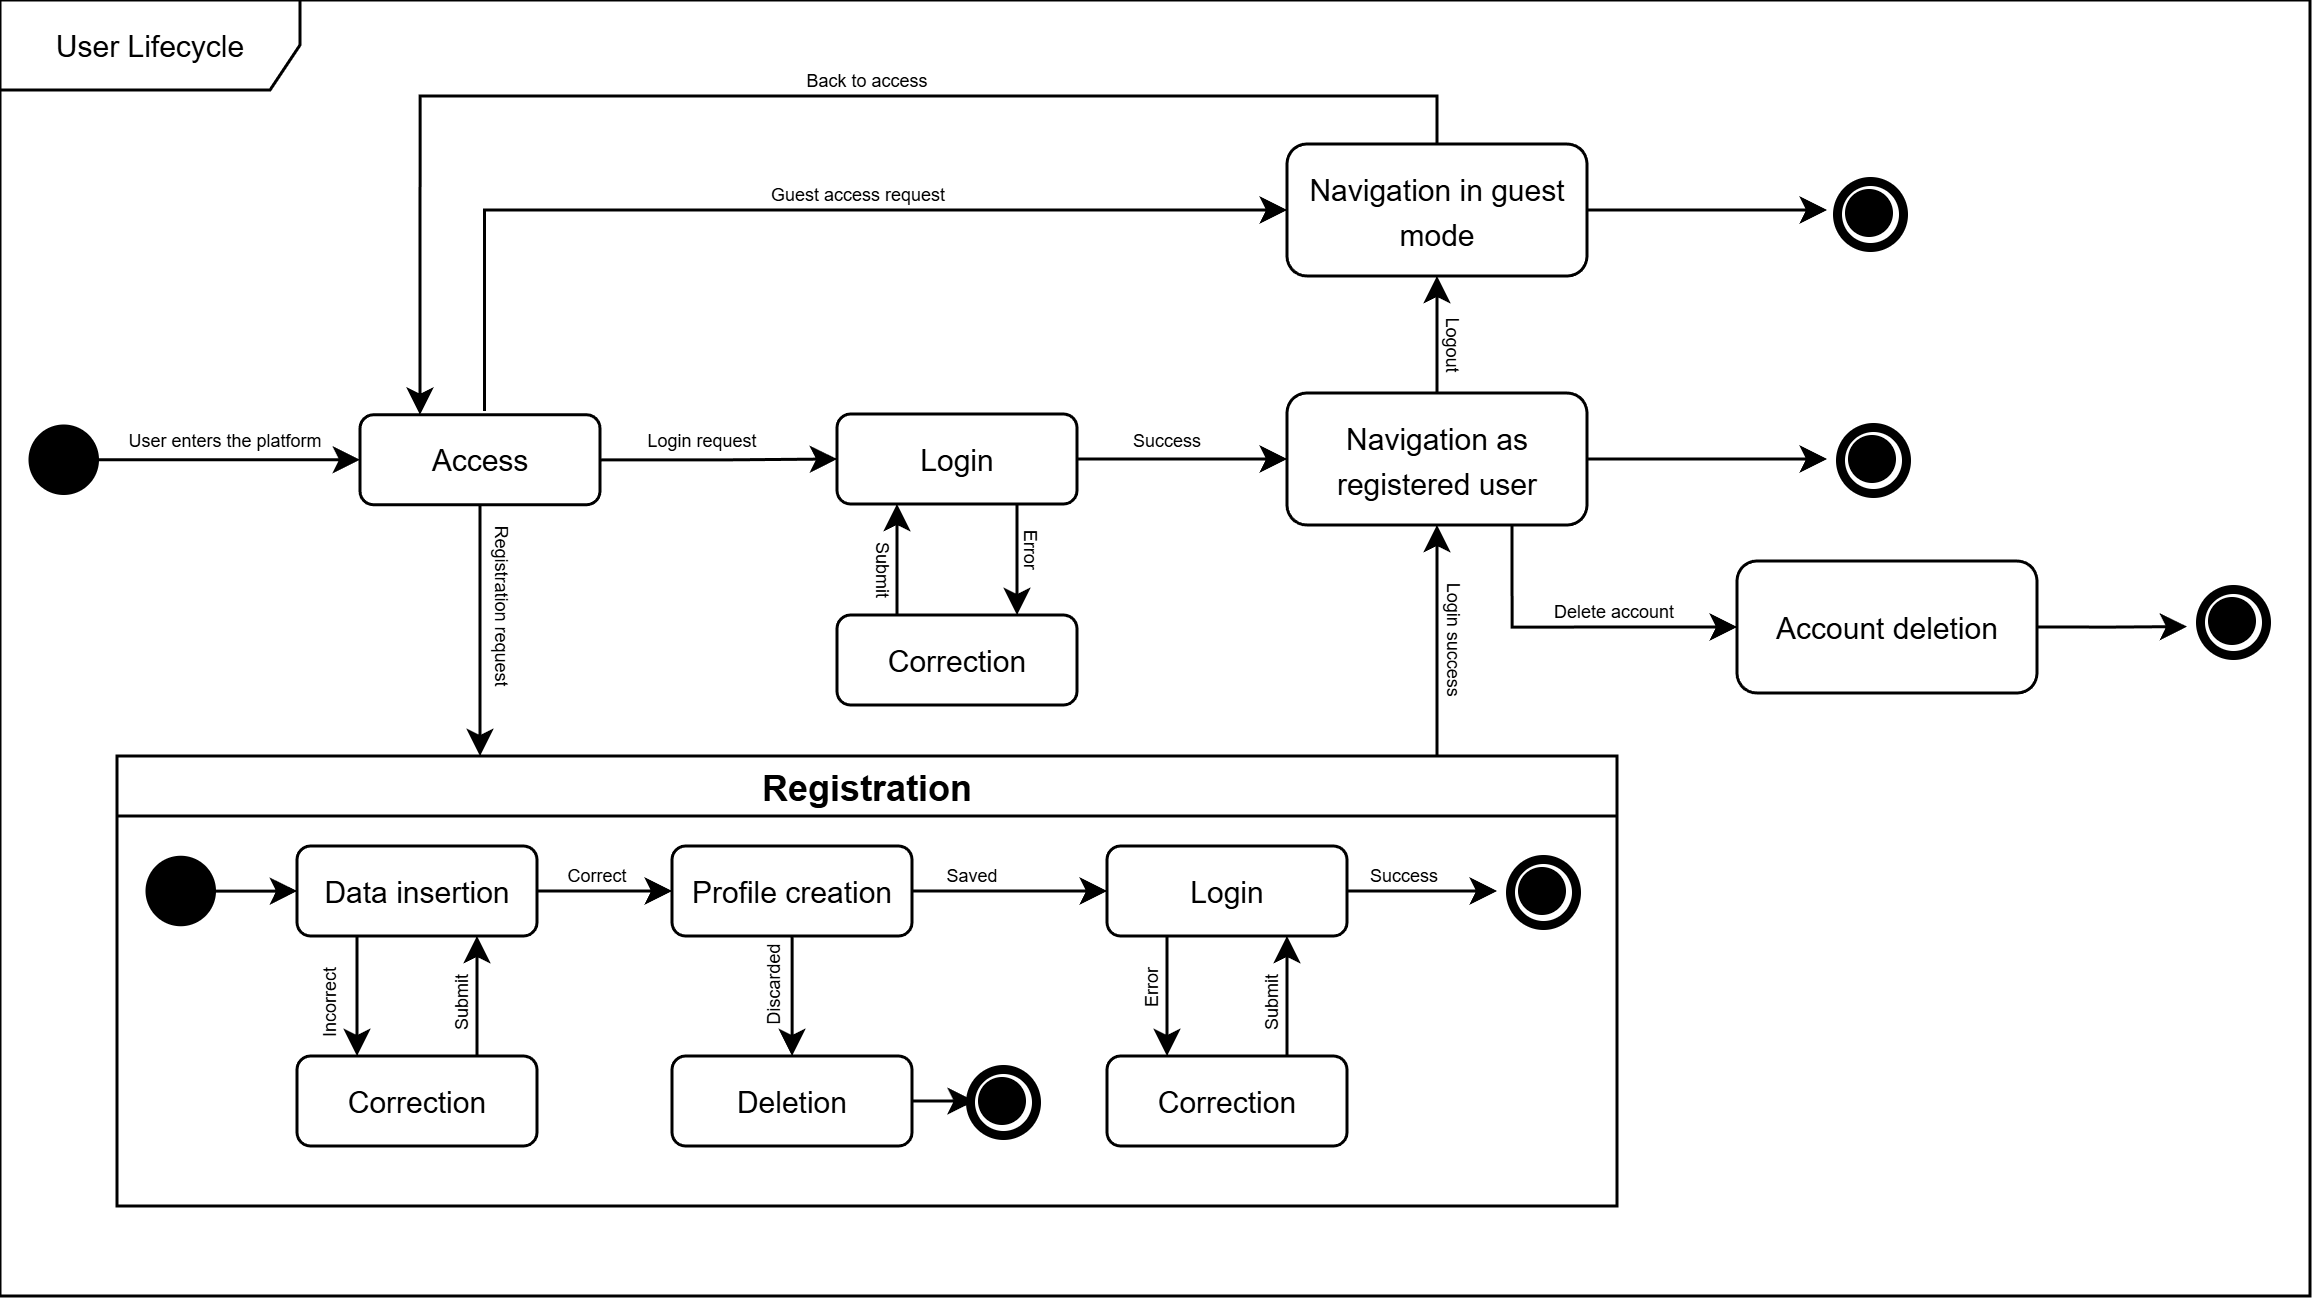
\includegraphics[width=1.5\textwidth]{images/userLifecycle.png}}

\newpage
\subsection{Product Functions}
\begin{enumerate}
    \item \textbf{Sign Up and Login}: when a user enters the BBP platform, they must be given the choice to login with their personal credentials if they already have an account. If they are not registered yet, they can either sign up or access the platform in guest mode. If the user decides to sign up, BBP collects and verifies the user's email address and asks to create a valid password.
    \item \textbf{Path registration in automated mode and possible publication}: this functionality is reserved for registered users who have successfully logged in. This mode is used to track the cycling session of the user and it must begin by asking the user to authorize BBP to access data collected by their mobile device's sensors. After receiving the necessary authorizations, the user must confirm that they want to use automated mode and only at this point the automatic retrieval and elaboration of data coming from the mobile device's GPS, gyroscope and accelerometer can begin. At the end of a session, the system should be able to successfully reconstruct the biker's path to determine when they have started or stopped cycling and when they have run into an obstacle by elaborating the retrieved data. The same data is also used to compute specific performance metrics (total distance, average speed, maximum speed, elevation gain, moving time and cadence). Once the elaboration is over, the system saves the session in the user's private log and immediately asks them if they want to publish it or just save it. In both cases, the system starts a guided process in which the user is asked to confirm the automatically calculated status of the streets and the presence of obstacles. At the end of the confirmation process, according to what the user chose to do, the system either shows a preview and allows them to publish the path or it shows the user the path in their private log.
    \item \textbf{Path registration and publication in manual mode}: this functionality is reserved for registered users who have successfully logged in. This mode is used to create and publish a path without relying on automatically retrieved data. To manually insert a path, the user is guided in inserting one by one the name of the streets that compose the path they have ridden along and their status. The insertion is performed by identifying the name of the street and visualizing it on a map and then asking the user to select the segment of the street that they have ridden along (in case the user does not specify anything, the segment corresponds to the whole street by default). For the insertion of the first street, in case a street with that name exists in different cities, the system shows the different option on a menu and waits for the user to select the correct one. The system keeps track of the city that has been specified and the beginning and performs a more restricted search for the following insertions. At each step, the system internally checks the validity of the user selection and, in case it detects an error (e.g. the selected street is not connected to the previous one), it asks them again for the name of the street and for the selection on the map. If the insertion goes well, the system also asks the user to rate the status of the path by choosing within a range of possible adjectives. At the end of the insertion process, the geographical accuracy of the path is checked again by BBP and, if the path is correct, a final user confirmation is needed to publish it. Note that correct paths that are not published by the user shall be discarded.
    \item \textbf{Private session visualization}: this functionality is reserved for registered users who have successfully logged in and it allows them to access the log of the paths that they have previously registered with automated mode. If the user who is the owner of a path has published that path, their associated performance metrics remain private and they are visible only in the user's personal log. If the path has not been published, the visibility of the performance metrics is the same as the previous case, but also the geographical reconstruction of the path, its status and the presence of obstacles remain private. In case the user has ridden along the same exact path multiple times, the system stores all the different records that contain the performance metrics associated to that path and makes them visible to the owner.
    \item \textbf{Path research}: this functionality is open to all users (registered or not) and it allows them to find existent paths between a specified origin and destination. When users access this functionality, they are asked and guided in inserting their starting and ending points. The system then takes care of browsing along all the published paths that exist and that suit the user's request and it then shows them on the map in an ordered manner, according to a calculated score. If no path exists, an error message is shown to the user. For existing paths, their score is obtained by subtracting a predefined number of points from an established maximum possible score for each obstacle (according to a measure of relevance) and for the streets' status. In case there are multiple suitable paths, the system visualizes a limited amount of them on the map. This amount can be modified by the user while staying in a predefined range. Note that paths are considered suitable for the user's query if their point of origin and destination match the user's specification with a certain degree of accuracy. This accuracy (radius expressed in meters) can be modified by the user and is set to 500 meters by default. If the user finds a path that they like, they can open it and visualize it in detail. If the wish, they can export it to a commercial maps app and receive real time navigation.
\end{enumerate}

\subsection{User Characteristics}
BBP's target users can generally be placed in one of the following user groups: 
\begin{itemize}
    \item \textbf{Amateur bikers}: these are more experienced bikers whose main purpose when cycling is training. 
    \item \textbf{Commuters and beginner bikers}: these users cycle mainly as a way to move around the city in their daily life (e.g. daily commute to the work place/university etc.).
    \item \textbf{Casual users}: these are users who are not interested in giving their active contribution; they just want to browse around and might want to access specific information.
\end{itemize}
These different categories of users use the platform for very different reasons and purposes, which means that they will likely be more interested in exploiting certain functionalities more than others. Here is a more detailed categorization of the user groups that have only been briefly defined above. Note that we will not go into details for the casual users who are not intended to be direct stakeholders for BBP.

\subsubsection{Amateur bikers}
\textbf{Users profile}\\
Amateur bikers are experienced bikers who have a strong passion for the sport. They train multiple times per week, have a deeper knowledge and understanding of technical aspects linked to the sport (specific terminology, biomechanical aspects, brand preferences etc.) and they usually own more sophisticated equipment. These users are also more likely to be interested in actively contributing to the bikers community as they directly have to deal with the difficulty of finding proper paths that satisfy their training needs. 

\vspace{0.5cm}
\noindent
\textbf{Educational level}\\
The general educational level of these individuals is not relevant to the use of the system but we assume that they have at least an intermediate level of domain-literacy. More specifically, we assume they are familiar with performance metrics that are commonly used in cycling such as average speed, elevation gain, cadence and moving time.

\vspace{0.5cm}
\noindent
\textbf{Experience with the system}\\
These users will likely use BBP almost on a daily basis, therefore, after overcoming the initial learning curve, they are expected to be proficient in the use of the platform and to maintain that proficiency overtime. 

\vspace{0.5cm}
\noindent
\textbf{Technical expertise}\\
Amateur bikers are used to tracking their sessions with mobile tracking devices that are frequently used in cycling such as smartwatches, heart rate monitors, cadence monitors and GPS. The consequent assumption is that these users own some kind of mobile device that has at least a built in GPS, accelerometer and gyroscope and that they know how to use it and how to place it on the bike.


\subsubsection{Commuters and beginner bikers}
\textbf{Users profile}\\
This category of users includes both beginner bikers who are new to the cycling world and commuters, who cycle almost daily as a way to get from one place to the other (e.g. to go to work or university). Both these kinds of cyclists might not always want to track their sessions since especially commuters are not interested in receiving performance metrics but only in paths memorization and discovery. These users usually do not own sophisticated gear besides their mobile phone and, in the average case, they will exploit contributions from other users more than what they will actively contribute.

\vspace{0.5cm}
\noindent
\textbf{Educational level}\\
The general educational level of these individuals is not relevant to the use of the system; we assume that they have very basic domain-literacy that mainly consists of notions that can be considered common and empirical knowledge even outside of the cycling world (e.g. notions of length of a path and capability to evaluate the quality of one).

\vspace{0.5cm}
\noindent
\textbf{Experience with the system}\\
These users will likely not use BBP on a daily basis which might slow down the process to become proficient.

\vspace{0.5cm}
\noindent
\textbf{Technical expertise}\\
These users do not generally have any specific technical expertise beyond the daily use of a mobile phone.

\subsubsection{Note on disabilities}
The intended user groups include cyclists with a wide range of physical and sensory capabilities. The user population is expected to include individuals with audio and visual impairments, specifically color vision deficiencies (CVD) and reduced visual acuity. Furthermore, users may possess motor and control limitations, either as permanent physical conditions or as situational constraints induced by the wearing of protective gear (e.g., thick gloves) and the vibration inherent to the cycling environment. These characteristics necessitate accommodations in the subsequent requirements regarding interface contrast, tactile feedback, and audio volume levels.

\subsection{Assumptions, Dependencies and Constraints}

\subsection{Domain assumptions}
\begin{itemize}
    \item DA1: The GPS, accelerometer and gyroscope of the biker's mobile device are functioning and they are able to provide data continuously.
    \item DA2: Bikers do not lie by providing invented information about paths they have not ridden along.
    \item DA3: Bikers provide true personal information if they register to the platform.
    \item DA4: Given two different paths, they are considered to have the same origin and destination if these two points in the two paths are within an acceptable distance radius from one another. 
    \item DA5: The meteorological information is actually relevant to the time and location of the biker.
    \item DA6: Bikers do not lie by signaling the presence of obstacles that are not there.
    \item DA7: Information provided by different bikers is considered mergeable if it regards the same street.
\end{itemize}

\subsection{Dependencies} %Dipendenze da servizi e/o fattori esterni
\begin{itemize}
    \item D1: The reconstruction of a path from GPS data and every other functionality that needs a geospatial infrastructure is possible through an external Map Service Provider.
    \item D2: Given a street, its speed limit or the average number of cars that travel along it is always a retrievable datum from the Map Service Provider.
    \item D3: Meteorological information is retrievable from an external MSP.
\end{itemize}



\subsection{Constraints} % Vincoli dati da condizioni esterne 
\begin{itemize}
    \item C1: Bikers are unable to use their hands to interact with the device while they cycle.
    \item C2: Bikers cannot safely look at their mobile device's screen while they cycle.
    \item C3: The environment around the biker could be too loud to allow them to hear audio coming from their mobile device.
    \item C4: Meteorological conditions might force the biker to have to put their mobile device away mid session to protect it.
    \item C5: Bikers might not own a proper support to mount their mobile device on the bike, therefore sensors readings might be particularly noisy.
    \item C6: Continuous GPS tracking significantly drains the mobile device battery.
    \item C7: Mobile device capabilities (quality of sensors, OS version, processor speed etc.) vary widely across the target user base.
\end{itemize}

\subsubsection{Policy and regulation constraints}
\begin{itemize}
    \item P\&R1: Adherence to fundamental road safety principles requires that the platform minimizes user workload and cognitive distraction to ensure safe operation of the bicycle.
    \item P\&R2: In compliance with GDPR, all collected data must be anonymized and protected against unauthorized access and disclosure.
    \item P\&R3: The platform shall provide support for all official languages, units of measure, and time formats for the target markets, ensuring compliance with multilingual support laws where required.
    \item P\&R4: The app shall adhere to all licensing terms and conditions for any embedded third-party software, including open-source libraries and commercial mapping APIs, and provide legally required copyright notices and attribution.
\end{itemize}

\newpage
\section{SPECIFIC REQUIREMENTS}
\subsection{External Interface Requirements}
\subsubsection{User Interfaces}
In this section we provide mockups of the application user interface. \\

\noindent The initial screen allows access either via login or in guest mode. Subsequent to selecting "Login" the option to register as a new user or enter existing credentials to access the platform as a registered user will be presented; however, the mockup for this specific transition screen is omitted. \\

\noindent The mockups subsequently emphasize the distinction between the feature set available in guest mode and the registered user mode. In the former, the sole available function is searching for a route within the path inventory. Conversely, the registered user mode additionally allows the user to track a new ride or review the log of previously completed rides.

\noindent\makebox[\textwidth][c]{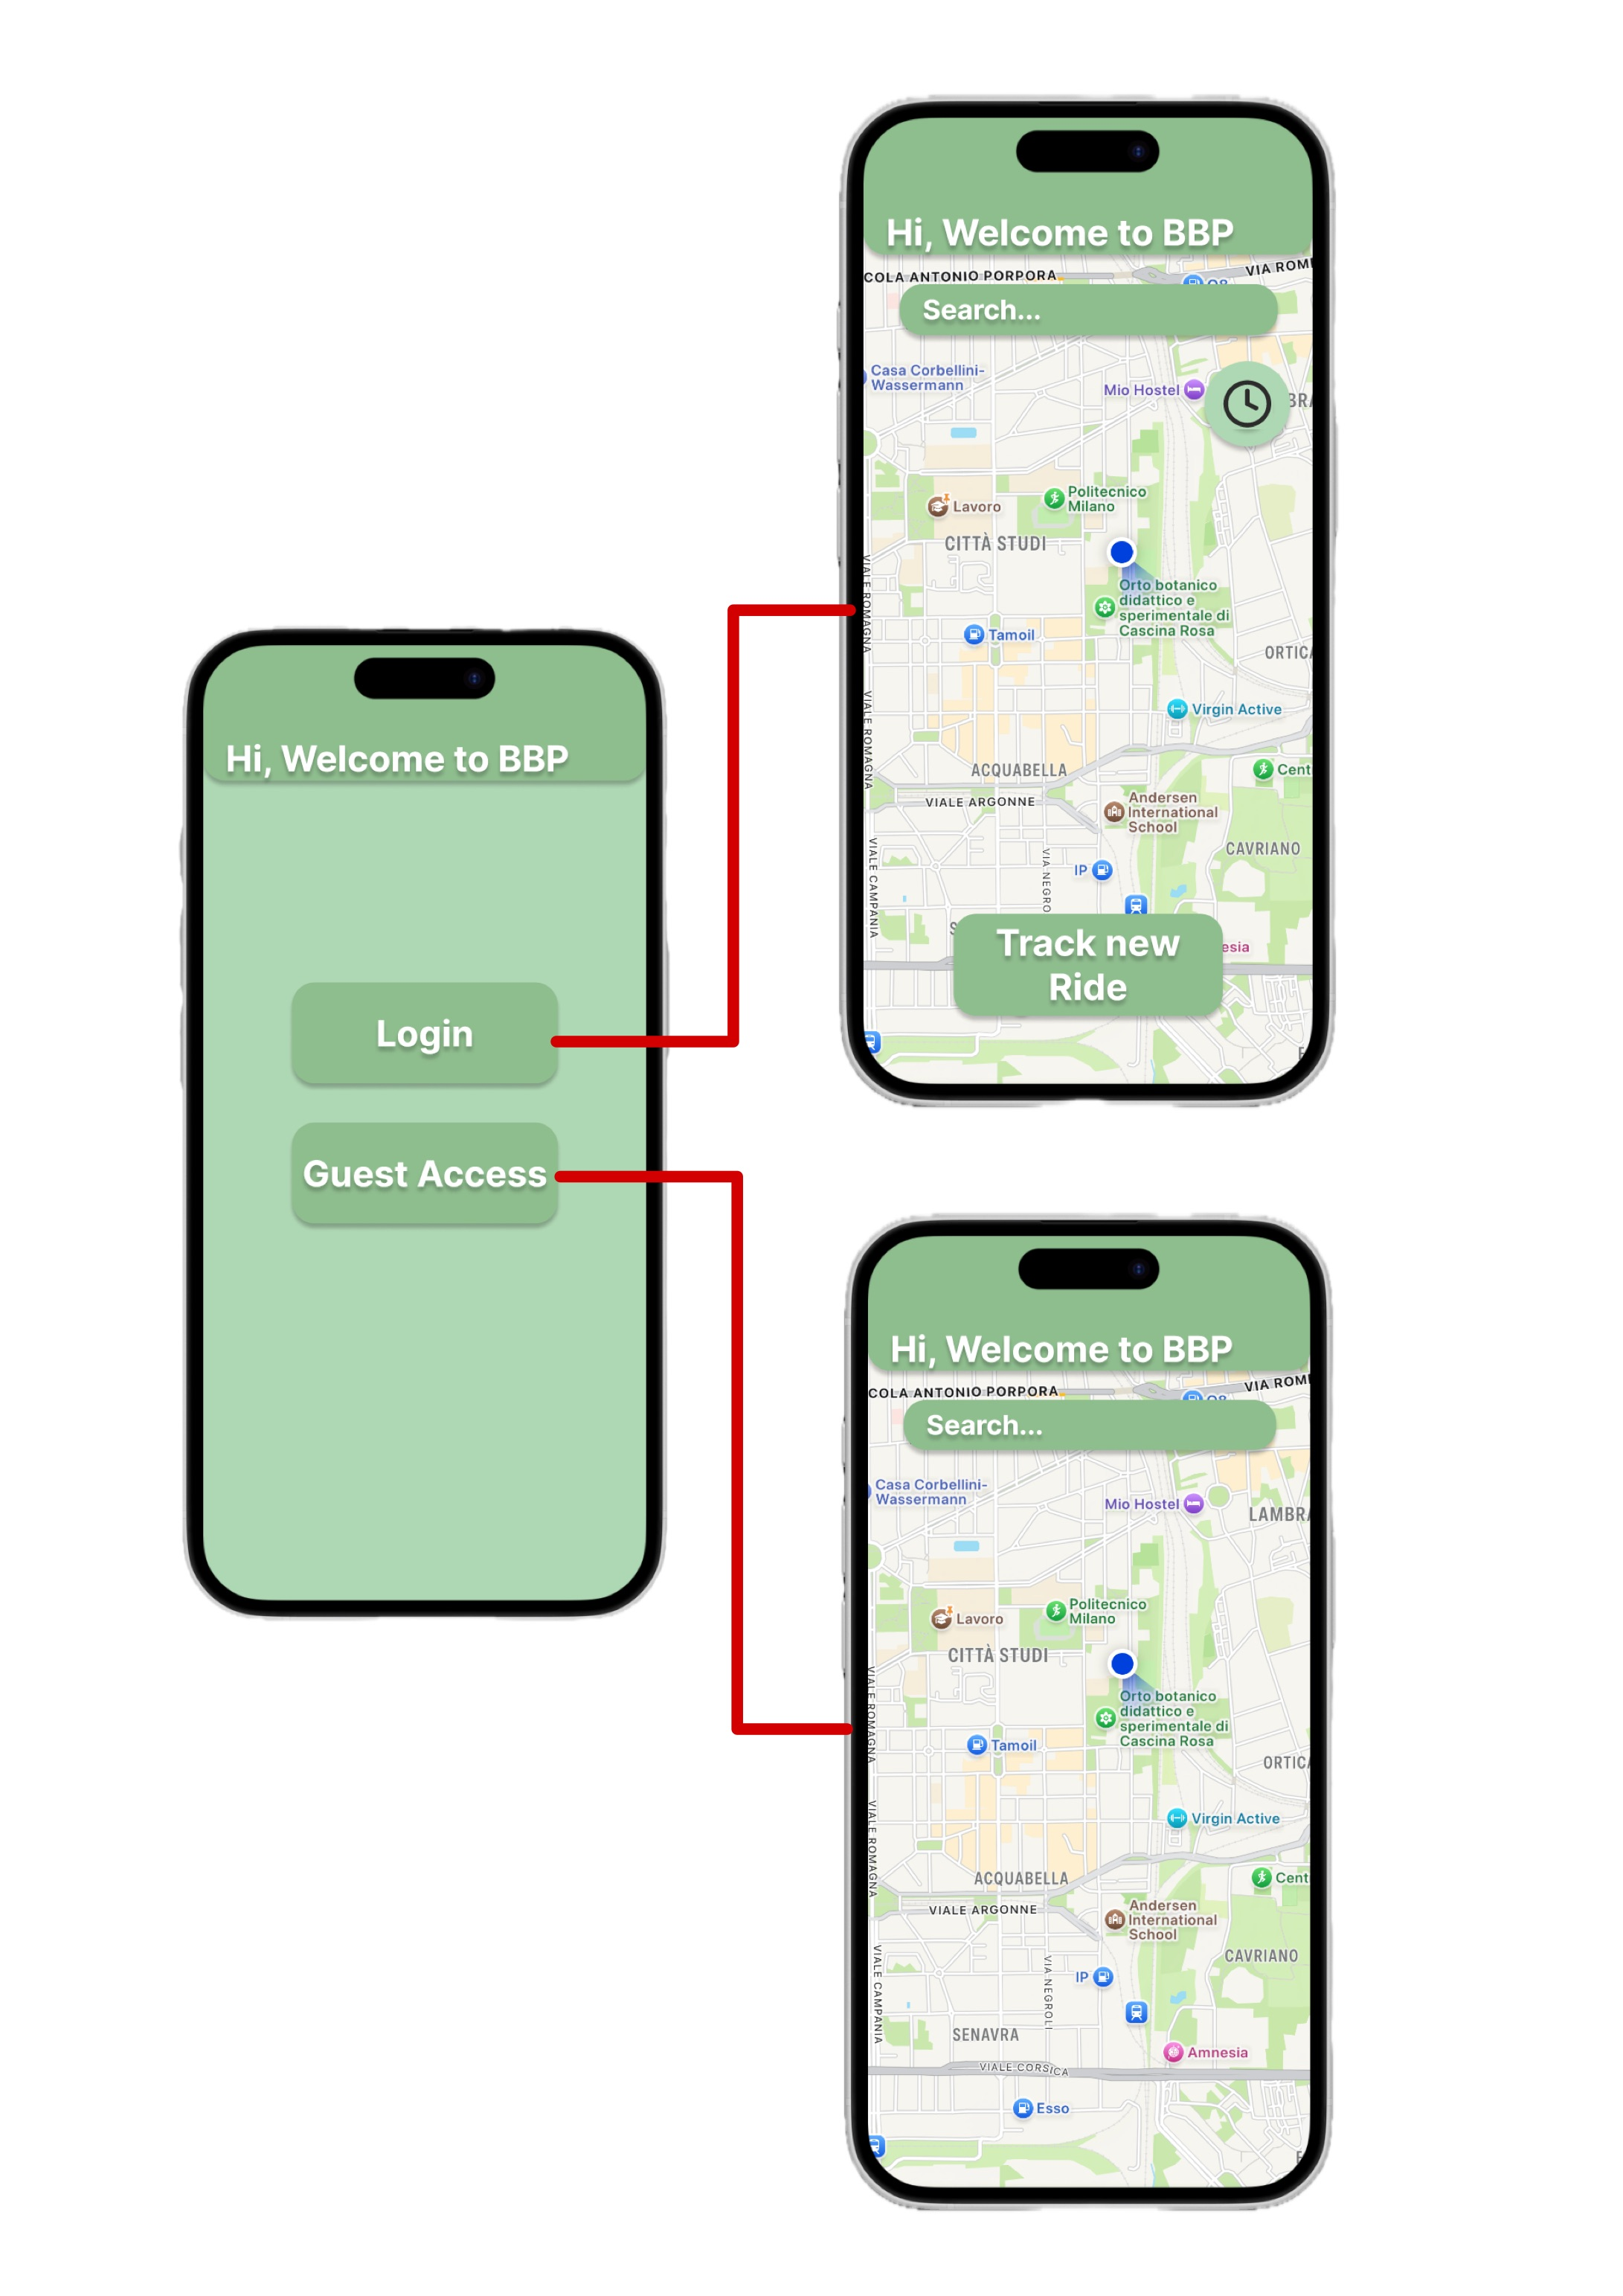
\includegraphics[width=0.7\textwidth]{images/prototipo1.jpg}}
\newline

The subsequent interfaces pertain exclusively to logged-in users' UI. A prototype illustrating the potential process for tracking a new ride in both manual and automatic modes is shown. \\

For manual mode, a screen is presented featuring a form to be completed with the ride's origin and destination. Furthermore, the travelled streets must be added in sequential order, along with their respective status. Upon finalizing the entry, the user can select either to "Confirm" or "Discard" the data. \\

Regarding automatic mode, a simple notification is displayed, confirming the initiation of tracking, alongside controls to "Stop" or "Terminate" the session. \\

Upon session termination, the user is redirected to the preview screen. This shared preview interface is common to both manual and automatic modes and displays a summary of all automatically collected or manually inserted data, offering the distinct option to publish the path. \\

In the case of an automatic session, after selecting "Publish," the system must allow the user to save the session exclusively to their private log. Publishing the path from this private log must then be enabled at a later time.

\noindent\makebox[\textwidth][c]{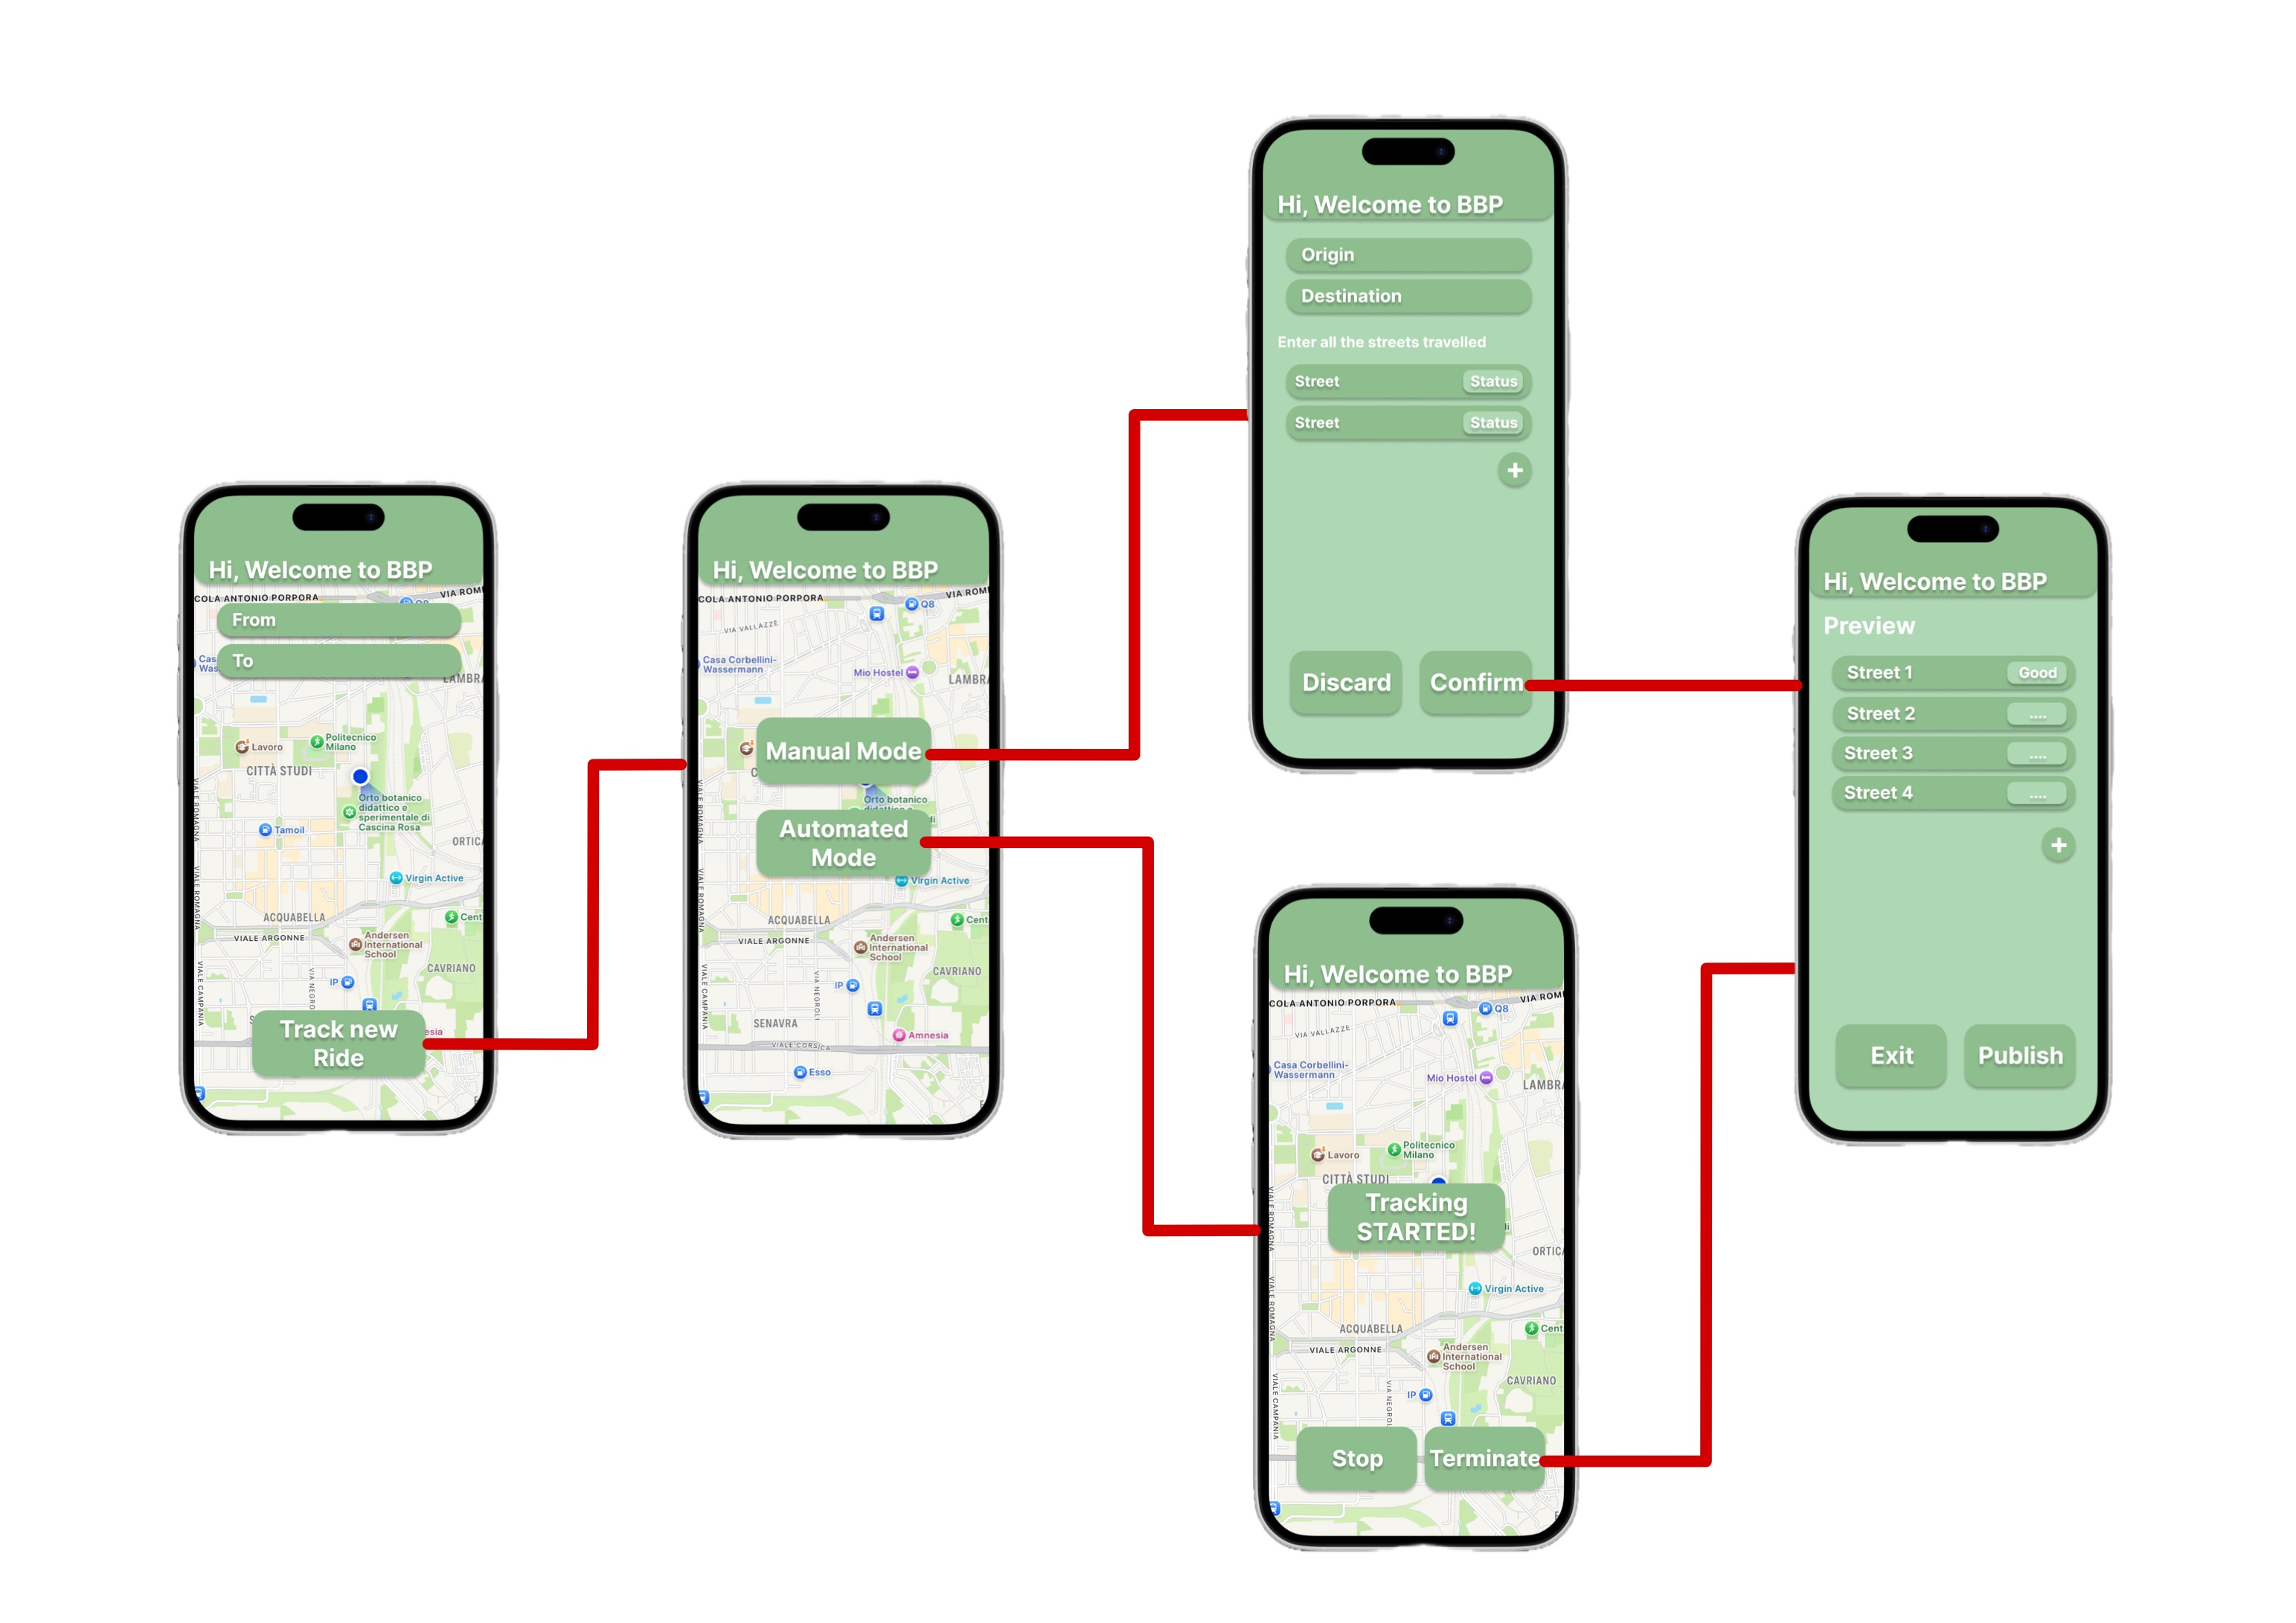
\includegraphics[width=1.2\textwidth]{images/prototipo2.jpg}}
Please note that the mockups are shown purely for illustrative purposes and to clarify the requested functional requirements. They are certainly not intended to be a guide that must be strictly adhered to.

\subsubsection{Hardware Interfaces}
The BBP software is designed to operate on standard smartphone devices. To execute its required functions, the application must interface with the following hardware components hosted on the user's device:

\begin{itemize}
    \item \textbf{GPS receiver}: the mobile application shall interface with the device's GPS receiver to retrieve real time geolocation data (latitude, longitude, and speed) for path reconstruction.
    \item \textbf{Accelerometer and gyroscope}: the application shall interface with the device's on board accelerometer and gyroscope sensors to detect vertical acceleration and orientation changes indicative of road irregularities (e.g., potholes).
    \item \textbf{Network interface}: the system shall utilize the mobile device’s wireless communication hardware (Cellular Data or Wi-Fi) to synchronize data with the central server and retrieve meteorological data from the external providers.
\end{itemize}

\subsubsection{Software Interfaces}
The BBP system requires specific software interfaces to support data acquisition, storage, and visualization. The following subsections describe the external libraries, APIs, operating systems, and database management systems that the BBP application must interface with to function correctly:

\begin{itemize}
    \item \textbf{MSP}: the system shall interface with a third party meteorological service to retrieve weather conditions, temperature, and wind speed to enrich recorded trip data with historical or real time weather context. BPP shall provide geolocation coordinates and a timestamp; the service shall return weather metrics in a standard format (e.g. JSON).
    \item \textbf{Map Service Provider}: The system shall interface with an external mapping provider (e.g. Google Maps API or OpenStreetMap) to geographically reconstruct and visualize paths from the GPS data. The system shall request map tiles, map matching and rendering services to display the reconstructed path and to identify markers for potholes or obstacles.
    \item \textbf{Database Management System (DBMS)}: the system shall utilize a relational or NoSQL database system to store registered user accounts, session records, bike path inventories, and statistical data. The backend system shall communicate with the DBMS using standard query languages (e.g. SQL) to perform Create, Read, Update, Delete (CRUD) operations.
    \item \textbf{Mobile Operating System}: the mobile application shall interface with the host Operating System (e.g. Android, iOS) to acquire sensor data (accelerometer, gyroscope) and GPS information from the hardware abstraction layer.
\end{itemize}

\vspace{0.5cm}
\noindent\makebox[\textwidth][c]{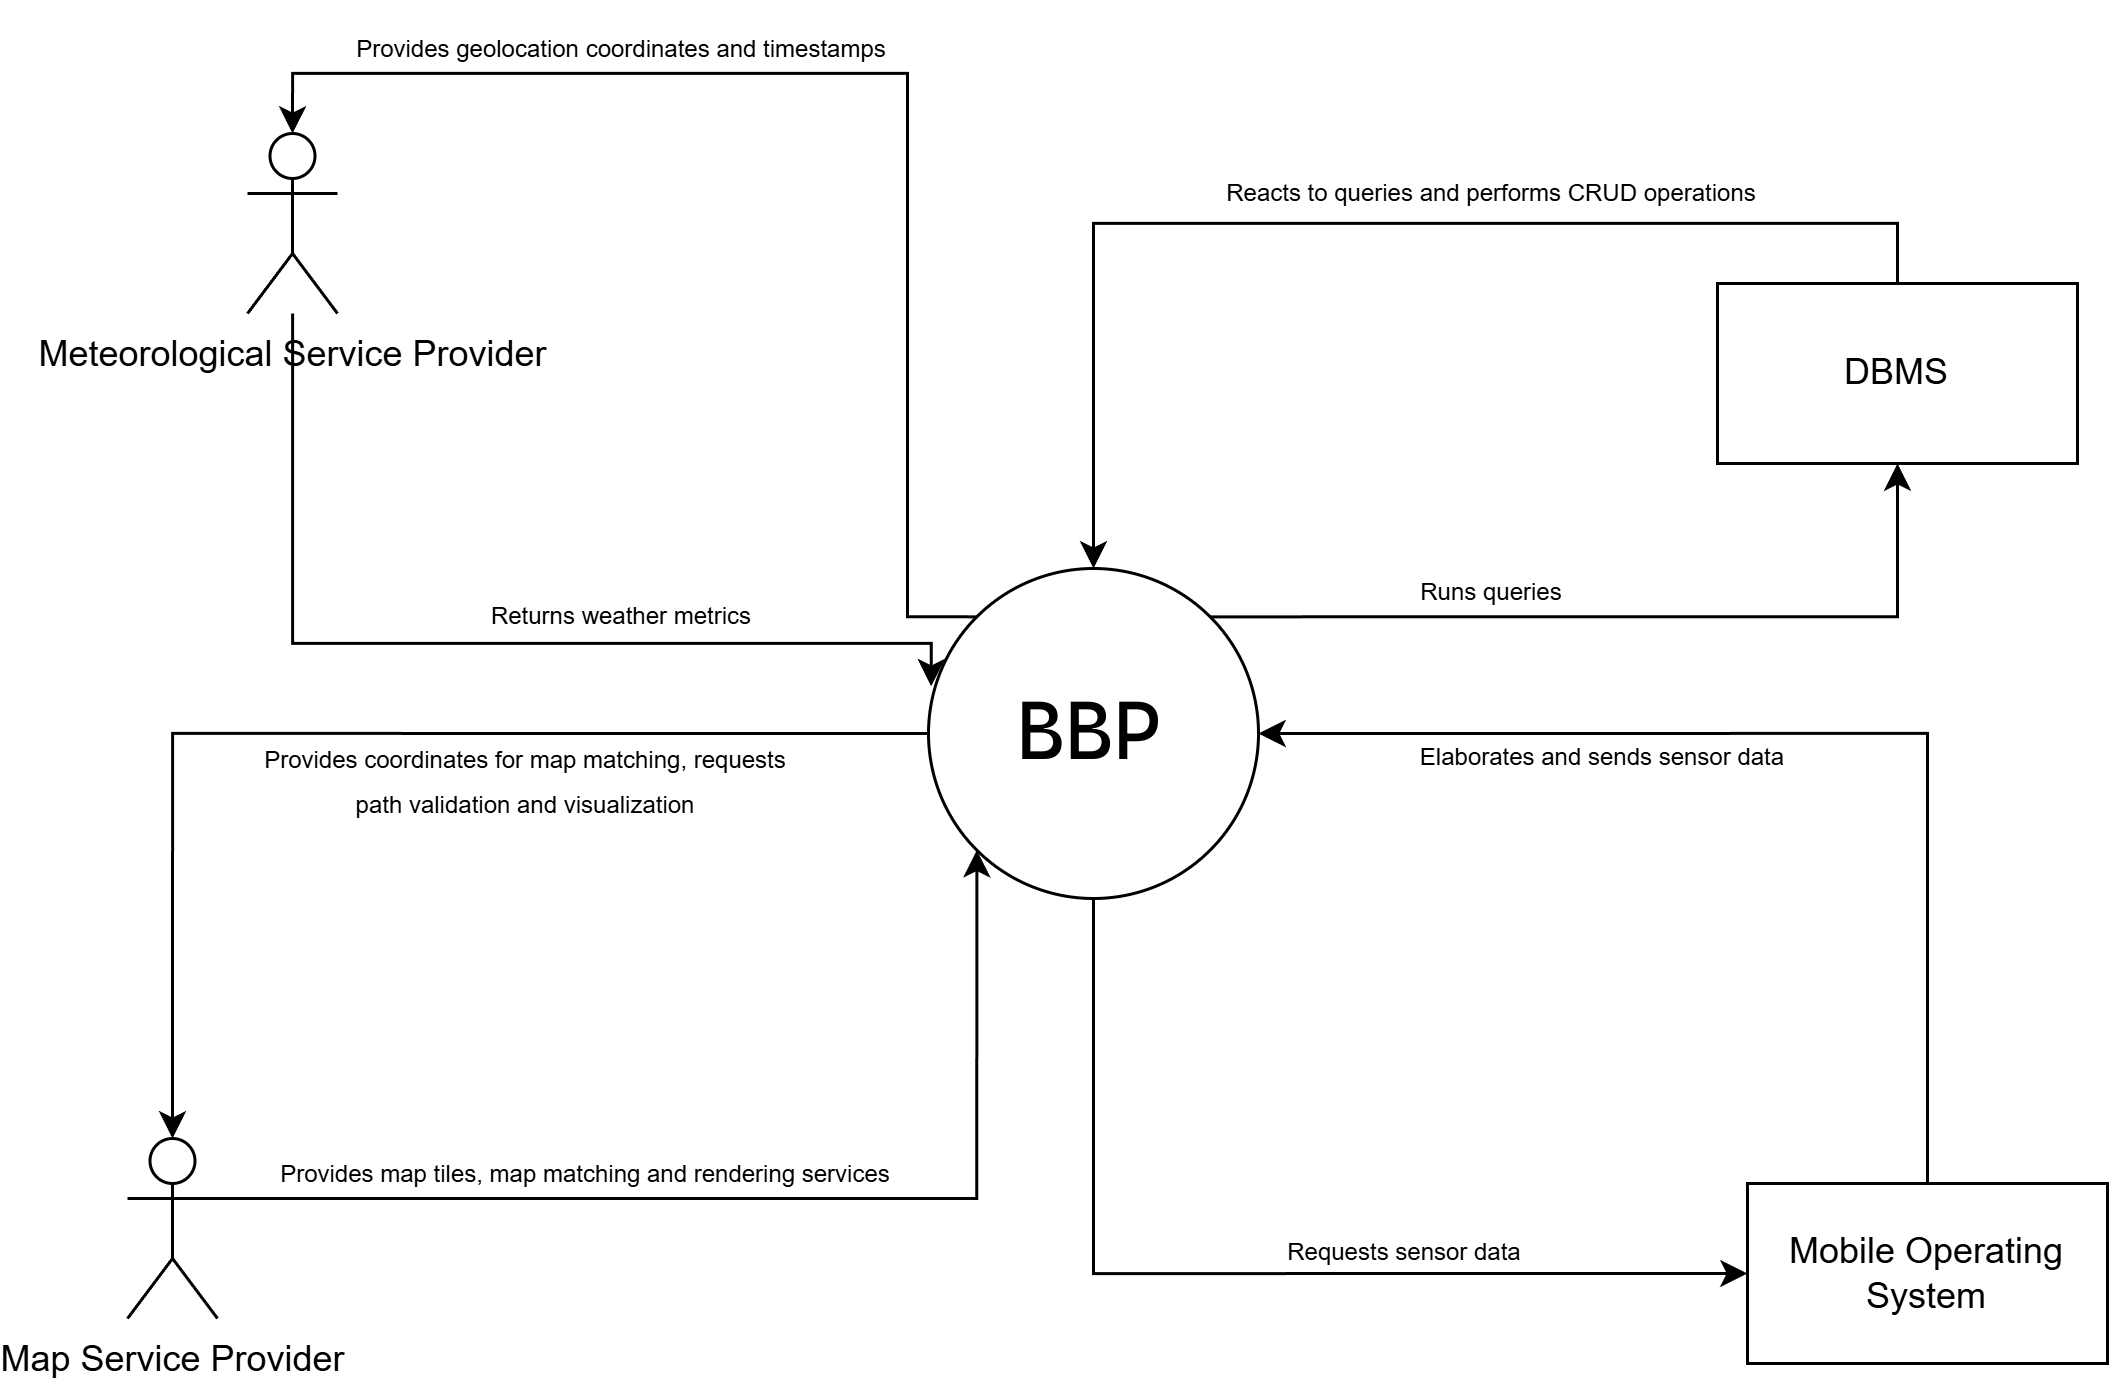
\includegraphics[width=1\textwidth]{images/contextDiagram.png}}

\subsubsection{Communication Interfaces}
This section specifies the communication protocols and standards required for data exchange between the BBP mobile application, the backend server, and external third-party services.
\begin{enumerate}
    \item \textbf{Communication Protocols}:
    \begin{itemize}
        \item \textbf{Client Server Interaction}: the mobile application shall communicate with the BBP backend server over the Internet using HTTPS (Hypertext Transfer Protocol Secure). This ensures that all sensitive data is encrypted during transmission.
        \item \textbf{Transport Layer}: all application-level data exchange shall occur over TCP/IP (Transmission Control Protocol/Internet Protocol) to ensure reliable delivery of trip segments and sensor data.
    \end{itemize}
    \item \textbf{Data Exchange Formats}:
    \begin{itemize}
        \item \textbf{API Payload}: data transferred between the mobile application and the server shall be serialized using JSON (JavaScript Object Notation) to ensure lightweight and efficient parsing on mobile devices.
        \item \textbf{External Services}: requests to the MSP shall adhere to the specific API standards provided by the vendor.
    \end{itemize}
    \item \textbf{Synchronization and Connectivity}
    \begin{itemize}
        \item \textbf{Asynchronous Transfer}: the system shall support asynchronous communication to allow trip data recording to continue locally on the device when network connectivity (Wi-Fi or Cellular) is unavailable, with synchronization occurring once connectivity is restored.
    \end{itemize}
\end{enumerate}

\subsection{Functional Requirements}

\textbf{ACCESS AND USERS MANAGEMENT}
\begin{itemize}
\item R1: BBP system allows users to create an account.
\item R2: BBP system must distinguish and manage authorization for registered and not registered users.
\end{itemize}

\noindent
\textbf{DATA ACQUISITION AND VALIDATION} 
\begin{itemize}
\item R3: BBP system shall enable a RU to initiate a trip tracking session.
\item R4: BBP system shall enable a RU to pause a trip tracking session.
\item R5: BBP system shall enable a RU to terminate a trip tracking session. 
\item R6: BBP system shall collect data from the mobile device’s GPS, gyroscope and accelerometer.
\item R7: BBP system shall geographically reconstruct the path that the user has ridden along from the GPS data that has been acquired in automated mode.
\item R8: BBP system shall use the data that has been acquired in automated mode to signal the possible presence of obstacles.
\item R9: In automated mode, BBP system shall monitor the biker’s speed to detect the start, pause and end of the activity.  
\end{itemize}

\noindent
\textbf{DATA MANAGEMENT AND PUBLICATION}
\begin{itemize}
\item R10: BBP system shall retrieve meteorological information from an external provider.
\item R11: BBP system shall receive a manual confirmation from the user before publishing data that has been acquired in automated mode.
\item R12: BBP system shall allow the RU to correct automatically identified data before publication.
\item R13: In manual mode, BBP system shall retrieve and validate the names and status of the streets that form the path that the RU has ridden along.
\item R14: BBP system shall publish the data that is manually submitted.
\item R15: BBP system shall keep a private log of tracked sessions for each RU that is only accessible from that user.
\end{itemize}

\noindent
\textbf{INFORMATION METRICS AND PATH SCORING}
\begin{itemize}
\item R16: BBP system shall compute and store the following performance metrics for a completed session: total distance covered, average speed, maximum speed, elevation gain, moving time and cadence.
\item R17: for each published path, BBP system shall calculate the path's score.
\item R18: the score of a path is computed by subtracting from the established maximum possible score a predefined number of points that depends on the individual streets' status and the relevance of the obstacles.
\item R19: BBP system shall display paths that match the user's request in order of score.
\end{itemize}

\noindent
\textbf{BROWSING AND MERGING}
\begin{itemize}
\item R20: BBP system shall display the existing paths whose origin and destination are within a predefined radius from the ones specified by the user.
\item R21: BBP system shall allow registered users to edit the accuracy radius within a certain range for their path queries.
\item R22: BBP system shall allow users to view all currently published path data, including their score.
\item R23: if multiple registered users have inserted information about the same street in different paths, BBP system shall internally merge the information and only show the result of the merge.
\item R24: the information merge performed by BBP shall consist of a computation that uses all the existing status values for the same streets and the insertion dates of the paths those streets are associated to.
\end{itemize}

\subsubsection{Use Case Diagrams}
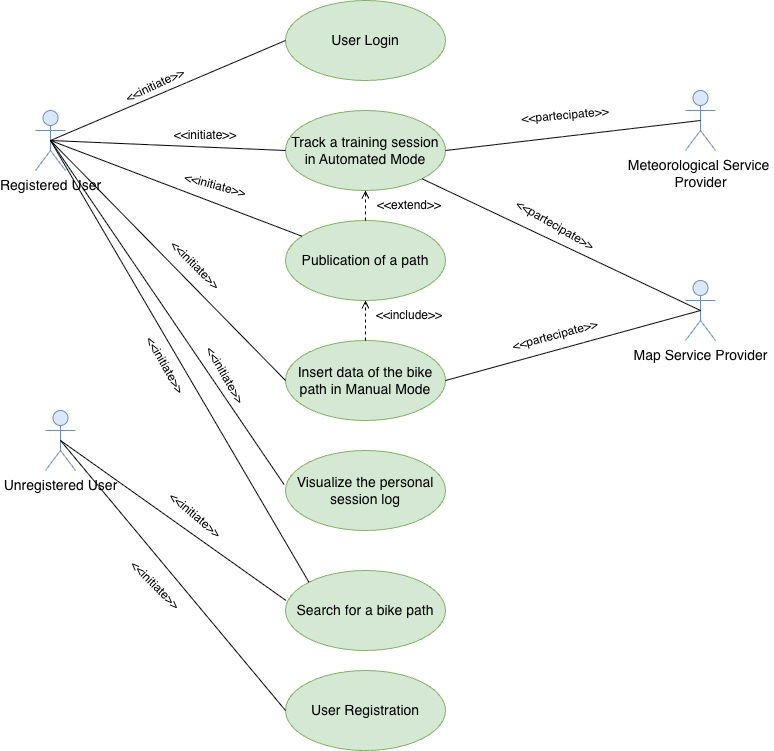
\includegraphics[width=1\textwidth ]{images/UseCaseDiagram.drawio.png}

\newpage
\subsubsection{Use Cases}
\textbf{[UC1] User Registration}
\begin{table}[H]
    \centering
    \begin{tabularx}{\textwidth}{|l|X|}
        \hline
        \textbf{Name} & \textbf{User Registration} \\
        \hline
        \textbf{Actors} & Unregistered User \\
        \hline
        \textbf{Entry Condition} & User opens the BBP platform \\
        \hline
        \textbf{Event Flow} & 
        (a) The user presses ``Sign up''. 
        \vspace{0.2cm}
        \newline
        (b) The system requires the user to fill out a form with their personal data.  
        \vspace{0.2cm}
        \newline
        (c) The system checks that the new user's data has not already been registered previously \\
        \hline
        \textbf{Exit Condition} & The user has successfully registered to the platform \\
        \hline
        \textbf{Exception} & (c) User is already registered on the platform \\
        \hline
    \end{tabularx}
    \caption{User Registration}
\end{table}

\textbf{[UC2] User Login}
\begin{table}[H]
    \centering
    \begin{tabularx}{\textwidth}{|l|X|}
        \hline
        \textbf{Name} & \textbf{User Login} \\
        \hline
        \textbf{Actors} & Registered User \\
        \hline
        \textbf{Entry Condition} & Registered User opens the BBP platform \\
        \hline
        \textbf{Event Flow} & 
        (a) The Registered User presses "Sign In"
        \vspace{0.2cm}
        \newline
        (b) The Registered User inserts their nickname or email. 
        \vspace{0.2cm}
        \newline
        (c) The Registered User inserts their password 
        \vspace{0.2cm}
        \newline
        (d) The system checks the data is correct \\
        \hline
        \textbf{Exit Condition} & The user has successfully logged in to the platform \\
        \hline
        \textbf{Exception} & (d) Data is not correct \\
        \hline
    \end{tabularx}
    \caption{User Login}
\end{table}

\newpage
\textbf{[UC3] Track a training session in Automated Mode}
\begin{table}[H]
    \centering
    \begin{tabularx}{\textwidth}{|l|X|}
        \hline
        \textbf{Name} & \textbf{Track a training session in Automated Mode} \\
        \hline
        \textbf{Actors} & Registered User, Meteorological Service Provider and Map Service Provider\\
        \hline
        \textbf{Entry Condition} & Registered User presses "Track new ride" to start a new ride\\
        \hline
        \textbf{Event Flow} & 
        (a) The Registered User presses "Start" to begin the tracking.
        \vspace{0.2cm}
        \newline
        (b) The system detects the User's position from their mobile device's GPS
        \vspace{0.2cm}
        \newline
        (c)  The system starts to keep track of the User's movement.
        \vspace{0.2cm}
        \newline
        (d) The system detects the end of the activity or the RU presses "Stop"
        \vspace{0.2cm}
        \newline
        (e) The system elaborates the retrieved data and shows a preview of the path to RU and waits for their validation
        \vspace{0.2cm}
        \newline
        (f) The RU checks and corrects status and obstacles data
        \\
        \hline
        \textbf{Exit Condition} & The RU presses "Save" or "Discard" \\
        \hline
    \end{tabularx}
    \caption{Track a training session in Automated Mode}
\end{table}

\textbf{[UC4] Insert data of the bike path in Manual Mode}
\begin{table}[H]
    \centering
    \begin{tabularx}{\textwidth}{|l|X|}
        \hline
        \textbf{Name} & \textbf{Insert data of the bike path in Manual Mode} \\
        \hline
        \textbf{Actors} & Registered User and Map Service Provider\\
        \hline
        \textbf{Entry Condition} & Registered User presses "Insert new ride" to manually register a new bike path.\\
        \hline
        \textbf{Event Flow} & 
        (a) The Registered User inserts the names and status of the streets that composed the path in order.
        \vspace{0.2cm}
        \newline
        (b) The system checks that the streets exist and form a path, in the given order.
        \vspace{0.2cm}
        \newline
        (c) The system shows a preview of the created path.
        \\
        \hline
        \textbf{Exit Condition} & The user presses "Save" or "Discard" \\
        \hline
        \textbf{Exception} & (a) Data is not correct \\
        \hline
    \end{tabularx}
    \caption{Insert data of the bike path in Manual Mode}
\end{table}

\newpage
\textbf{[UC5] Visualize a session in the personal sessions log}
\begin{table}[H]
    \centering
    \begin{tabularx}{\textwidth}{|l|X|}
        \hline
        \textbf{Name} & \textbf{Visualize a session in the personal sessions log} \\
        \hline
        \textbf{Actors} & Registered User\\
        \hline
        \textbf{Entry Condition} & The RU selects "My recorded trips"\\
        \hline
        \textbf{Event Flow} & 
        (a) The system shows the sessions log
        \vspace{0.2cm}
        \newline
        (b) The RU finds the session they are interested in and selects it.
        \vspace{0.2cm}
        \newline
        (c) The system shows the details of the selected sessions.
        \\
        \hline
        \textbf{Exit Condition} & The RU presses "Exit" \\
        \hline
    \end{tabularx}
    \caption{Visualize a session in the personal sessions log}
\end{table}

\textbf{[UC6] Search for a bike path}
\begin{table}[H]
    \centering
    \begin{tabularx}{\textwidth}{|l|X|}
        \hline
        \textbf{Name} & \textbf{Search for a bike path} \\
        \hline
        \textbf{Actors} & Registered User or Unregistered User\\
        \hline
        \textbf{Entry Condition} & The User presses "Search" to find a path\\
        \hline
        \textbf{Event Flow} & 
        (a) The system detect the User's position from their mobile device's GPS
        \vspace{0.2cm}
        \newline
        (b) The User chooses if they want to use the detected position or another one.
        \vspace{0.2cm}
        \newline
        (c) The User chooses their destination.
        \vspace{0.2cm}
        \newline
        (d) The system shows a selection of published paths that match the User's desired origin and destination. 
        \vspace{0.2cm}
        \newline
        (e) The User chooses their desired path.
        \\
        \hline
        \textbf{Exit Condition} & The user presses "View" or "Exit"\\
        \hline
    \end{tabularx}
    \caption{Search for a bike path}
\end{table}

\textbf{[UC7] Visualization of a path}
\begin{table}[H]
    \centering
    \begin{tabularx}{\textwidth}{|l|X|}
        \hline
        \textbf{Name} & \textbf{Visualization of a path} \\
        \hline
        \textbf{Actors} & Registered User or Unregistered User\\
        \hline
        \textbf{Entry Condition} & The User has performed a path search and the BBP system has provided a selection of published paths that match their query. The User has then selected a specific path and pressed "View".\\
        \hline
        \textbf{Event Flow} & 
        (a) The system shows the details of the selected path.
        \\
        \hline
        \textbf{Exit Condition} & The user presses "Exit"\\
        \hline

    \end{tabularx}
    \caption{Visualization of a path}
\end{table}

\textbf{[UC8] Publication of a path}
\begin{table}[H]
    \centering
    \begin{tabularx}{\textwidth}{|l|X|}
        \hline
        \textbf{Name} & \textbf{Publication of a path} \\
        \hline
        \textbf{Actors} & Registered User\\
        \hline
        \textbf{Entry Condition} & The RU presses "Publish" to make a path available on the public paths inventory.\\
        \hline
        \textbf{Event Flow} & 
        (a) The system shows a preview of the path and its related publishable data.
        \vspace{0.2cm}
        \newline
        (b) The system waits for the Registered User's final confirmation.
        \\
        \hline
        \textbf{Exit Condition} & The user presses "Confirm" or "Exit"\\
        \hline 
    \end{tabularx}
    \caption{Publication of a path}
\end{table}


\subsubsection{Sequence Diagrams}
\noindent\makebox[\textwidth][c]{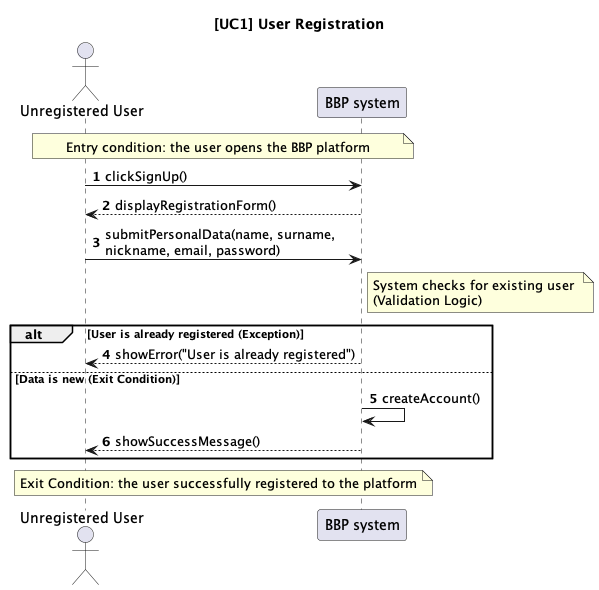
\includegraphics[width=1\textwidth]{images/UC1_UserRegistration_RASD.png}}

\noindent\makebox[\textwidth][c]{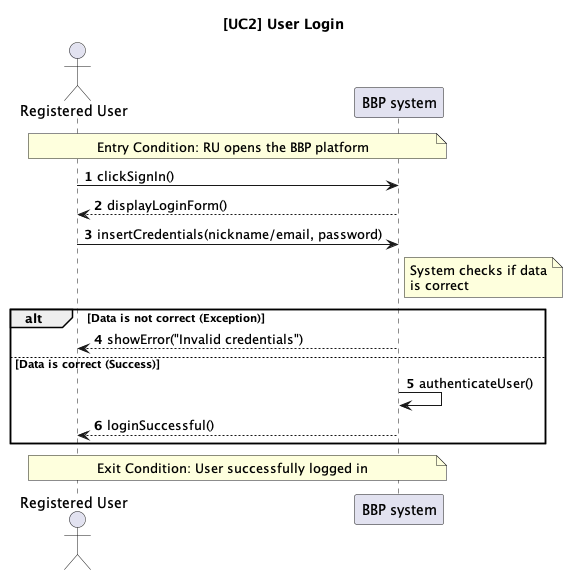
\includegraphics[width=1\textwidth]{images/UC2_UserLogin_RASD.png}}

\noindent\makebox[\textwidth][c]{\includegraphics[width=1\textwidth]{images/UC3_AutomatedMode_RASD.png}}

\noindent\makebox[\textwidth][c]{\includegraphics[width=1\textwidth]{images/UC4_ManualMode_RASD.png}}

\noindent\makebox[\textwidth][c]{\includegraphics[width=1\textwidth]{images/UC5_ReviewPath_RASD.png}}

\noindent\makebox[\textwidth][c]{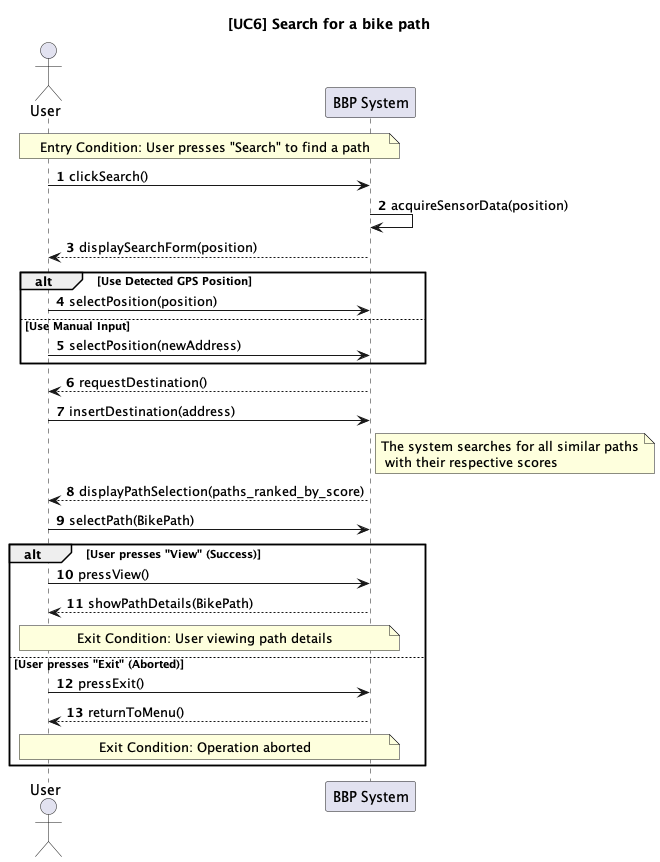
\includegraphics[width=1\textwidth]{images/UC6_SearchBikePath_RASD.png}}

\noindent\makebox[\textwidth][c]{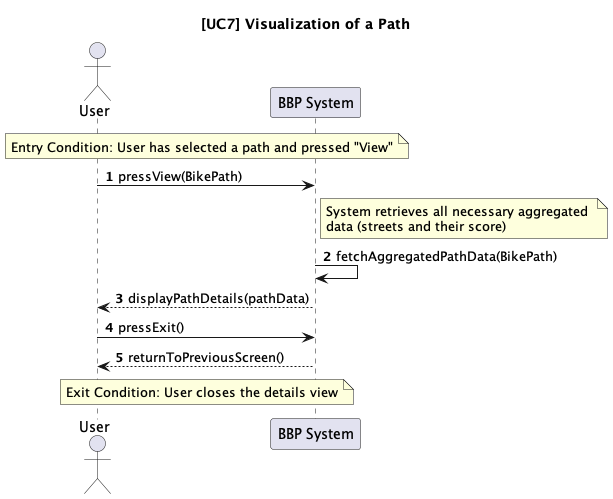
\includegraphics[width=1\textwidth]{images/UC7_VisualizationPath_RASD.png}}

\noindent\makebox[\textwidth][c]{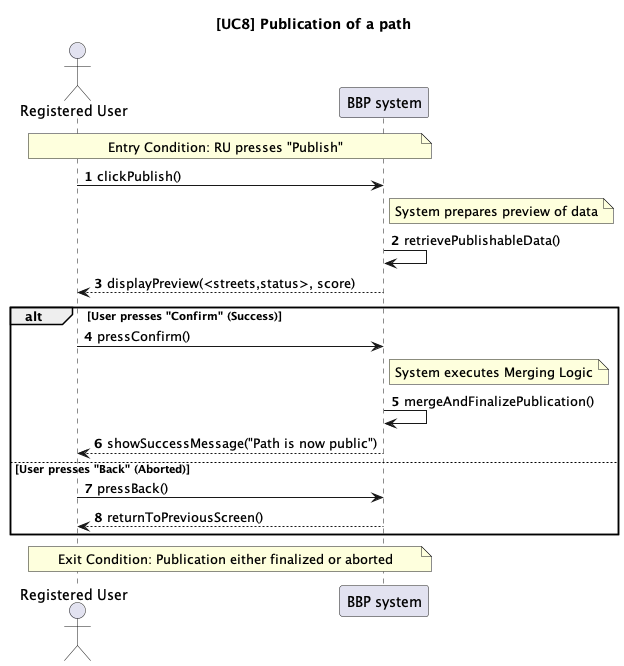
\includegraphics[width=1\textwidth]{images/UC8_PublicationPath_RASD.png}}

\newpage
\subsubsection{Requirement Mapping}

%G1 requirement mapping
\begin{xltabular}{\textwidth}{|X|X|}
    \hline
    \multicolumn{2}{|p{\dimexpr\textwidth-2\tabcolsep-2\arrayrulewidth}|}{
        \textbf{G1:} Bikers share a path that they have ridden along with other bikers.
    } \\
    \hline
 
    R1: BBP allows users to create an account \par
    R2: BBP system must distinguish and manage authorization for registered and not registered users \par
    R6: BBP system shall collect data from the mobile device’s GPS, gyroscope and accelerometer \par
    R7: BBP system shall geographically reconstruct the path that the user has ridden along from the GPS data that has been acquired in automated mode. \par
    R8: BBP system shall use the data that has been acquired in automated mode to signal the possible presence of obstacles. \par
    R9: In automated mode, BBP system shall monitor the biker’s speed to detect the start, pause and end of the activity \par
    R10: BBP system shall retrieve meteorological information from an external provider \par
    R11: BBP system shall receive a manual confirmation from the user before publishing data that has been acquired in automated mode \par
    R12: BBP system shall allow the RU to correct automatically identified data before final confirmation \par
    R13: In manual mode, BBP system shall retrieve and validate the names and status of the streets that form the path that the RU has ridden along. \par
    R14: BBP system shall publish the data that is manually submitted 
    & 
    DA1: The GPS, accelerometer and gyroscope of the biker’s mobile device are functioning and they are able to provide data continuously. \par
    DA2: Bikers do not lie by providing invented information about paths they have not ridden along. \par
    DA6: Bikers do not lie by signaling the presence of obstacles that are actually not there. \par
    DA7: Information provided by different bikers is considered mergeable if it regards the same street.
    \\
    \hline
    R20: BBP system shall display the existing paths whose origin and destination are within a predefined radius from the ones specified by the user. \par
    R21: BBP system shall allow registered users to edit the accuracy radius within a certain range for their path queries.  \par
    R22: BBP system shall allow users to view all currently published path data, including their score. \par
    R23: if multiple registered users have inserted information about the same street in different paths, BBP system shall internally merge the information and only show the result of the merge. \par
    R24: the information merge performed by BBP shall consist of a computation that uses all the existing status values for the same streets and the insertion dates of the paths those streets are associated to.
    & \par
    \\
    \hline
\end{xltabular}

\newpage
%G2 requirement mapping
\begin{xltabular}{\textwidth}{|X|X|}
    \hline
    \multicolumn{2}{|p{\dimexpr\textwidth-2\tabcolsep-2\arrayrulewidth}|}{
        \textbf{G2:} Bikers give other bikers information about the status and the presence of obstacles on paths that they have ridden along.
    } \\
    \hline
 
    R1: BBP allows users to create an account \par
    R2: BBP system must distinguish and manage authorization for registered and not registered users \par
    R6: BBP system shall collect data from the mobile device’s GPS, gyroscope and accelerometer \par
    R7: BBP system shall geographically reconstruct the path that the user has ridden along from the GPS data that has been acquired in automated mode. \par
    R8: BBP system shall use the data that has been acquired in automated mode to signal the possible presence of obstacles. \par
    R10: BBP system shall retrieve meteorological information from an external provider \par
    R11: BBP system shall receive a manual confirmation from the user before publishing data that has been acquired in automated mode \par
    R12: BBP system shall permit the RU to correct automatically identified data before final confirmation 
    & 
    DA1: The GPS, accelerometer and gyroscope of the biker’s mobile device are functioning and they are able to provide data continuously.   \par
    DA2: Bikers do not lie by providing invented information about paths they have not ridden along. \par
    DA3: Bikers provide true personal information if they register to the platform. \par
    DA6: Bikers do not lie by signaling the presence of obstacles that are actually not there. \par
    \\
    %\hline
    R13: In manual mode, BBP system shall retrieve and validate the names and status of the streets that form the path that the RU has ridden along. \par
    R14: BBP system shall publish the data that is manually submitted \par
    R20: BBP system shall display the existing paths whose origin and destination are within a predefined radius from the ones specified by the user.  & 
    \\
    \hline
\end{xltabular}

\newpage
%G3 requirement mapping
\begin{xltabular}{\textwidth}{|X|X|}
    \hline
    \multicolumn{2}{|p{\dimexpr\textwidth-2\tabcolsep-2\arrayrulewidth}|}{
        \textbf{G3:} Bikers are able to track and record their cycling trips to maintain a log of their activity that contains relevant information about their performance.
    } \\
    \hline
 
    R1: BBP allows users to create an account \par
    R2: BBP system must distinguish and manage authorization for registered and not registered users \par
    R3: BBP system shall enable a RU to initiate a trip tracking session \par
    R4: BBP system shall enable a RU to pause a trip tracking session \par
    R5: BBP system shall enable a RU to terminate a trip tracking session
    R6: BBP system shall collect data from the mobile device’s GPS, gyroscope and accelerometer \par
    R7: BBP system shall geographically reconstruct the path that the user has ridden along from the GPS data that has been acquired in automated mode. \par
    R8: BBP system shall use the data that has been acquired in automated mode to signal the possible presence of obstacles. 
    & 
    DA1: The GPS, accelerometer and gyroscope of the biker’s mobile device are functioning and they are able to provide data continuously.   \par
    DA3: Bikers provide true personal information if they register to the platform. \par
    DA5: The meteorological information is actually relevant to the time and location of the biker. \\
    R9: In automated mode, BBP system shall monitor the biker’s speed to detect the start, pause and end of the activity \par
    R10: BBP system shall retrieve meteorological information from an external provider \par
    R15: BBP system shall store and permit access to a log of tracked sessions for the RU \par
    R16: The BBP system shall compute performance metrics for a completed trip (e.g., total distance covered, average speed, maximum speed, elevation gain, moving time and cadence) & \par
    \\
    \hline

\end{xltabular}

\newpage
%G4 requirement mapping
\begin{xltabular}{\textwidth}{|X|X|}
    \hline
    \multicolumn{2}{|p{\dimexpr\textwidth-2\tabcolsep-2\arrayrulewidth}|}{
        \textbf{G4:} Bikers are presented with a set of paths, comprehensive of information about the path’s status and navigational efficiency, between a specified origin and destination.
    } \\
    \hline
 
    R17: BBP system shall calculate the path score which is based on the status of the streets that composed the path and based on bikers’ opinion too \par
    R18: BBP system shall display similar paths ordered by their score \par
    R19: BBP system shall display paths that match the user's request in order of score. \par
    R20: BBP system shall display the existing paths whose origin and destination are within a predefined radius from the ones specified by the user. \par
    R21: BBP system shall merge information about the same streets in different paths \par
    R22: BBP must merge the published information considering the date of publication and the number of data that are equivalent
    & 
    DA4: Given two different paths, they are considered to have the same origin and destination if these two points in the two paths are within an acceptable distance radius from one another.   \par
    DA7: Information provided by different bikers is considered mergeable if it regards the same street. \\
    \hline

\end{xltabular}

\newpage
\subsection{Performance Requirements}
In this section we provide an overview of the static and dynamic numerical requirements placed on the software and/or the human interaction with it that are necessary for the application to run smoothly.

\begin{itemize}
    \item \textbf{Sensor data acquisition}: the app shall be capable of sampling accelerometer and gyroscope data at a minimum frequency of 50 Hz to ensure accurate detection of road surface anomalies while the user is biking.
    \item \textbf{Data synchronization}: the system shall be capable of synchronizing a completed trip log to the central server within 30 seconds upon establishing a stable network connection.
    \item \textbf{Concurrent users}: the system shall support concurrent recording of trips and data transmission for a minimum number of users without degrading response times below a defined threshold.
    \item \textbf{Path visualization}: the system shall calculate and render a bike path within 3 seconds of the request under normal network conditions (4G/LTE or Wi-Fi).
\end{itemize}

\subsection{Design Constraints}
In this section, we go more into depth about constraints on the system design that are imposed by external standards, regulatory requirements or other limitations.
\subsubsection{Standards Compliance}
\begin{itemize}
    \item \textbf{Data privacy (GDPR)}: the system shall comply with the General Data Protection Regulation (GDPR) regarding the collection, storage, and processing of personal geolocation data. Users must explicitly consent to location tracking and have the "right to be forgotten" (deletion of trip history).
    \item \textbf{Map standards}: the system shall utilize standard geospatial data formats for the representation and exchange of path coordinates and map layers to ensure compatibility with external mapping services.
    \item \textbf{Security protocols}: all data transmission between the mobile client and the server shall adhere to TLS 1.3 (Transport Layer Security) standards to protect user credentials and trip data.
\end{itemize}
\subsubsection{Hardware Limitations}
\begin{itemize}
    \item \textbf{Battery consumption}: the mobile application shall optimize the usage of the GPS receiver and background sensors (accelerometer/gyroscope) to not exceed 15\% of the device's battery capacity per hour of active trip recording.
    \item \textbf{Storage constraints}: the mobile application shall use no more than 500 MB of local storage on the user's device for caching map tiles and temporary trip logs before synchronization.
\end{itemize}
\subsubsection{Any Other Constraint}
\begin{itemize}
    \item \textbf{Network intermittency}: the mobile application must be designed to function in an "offline-first" manner, caching sensor and location data locally when the user enters areas with poor cellular coverage (e.g., rural bike paths) and synchronizing once connectivity is restored.
    \item \textbf{Device orientation}: the user shall be instructed on how to properly place the device to acquire data accurately in automated mode.
\end{itemize}

\subsection{Software System Attributes}
In this section we specify the required quality attributes of the software product.
\subsubsection{Reliability}
The system shall prevent data loss in the event of an application crash or device power failure during a trip. The application must periodically auto-save trip segments locally to be able to reconstruct the path.
\subsubsection{Availability}
The BBP backend server (composed of the APIs and the DBMS) shall be available 99.9\% of the time during scheduled service hours to ensuring users can upload trips and query paths when needed.
\subsubsection{Security}
The system shall ensure that users can only modify or delete their own trip data. Publishable information must be anonymized before being aggregated into the public map view to prevent stalking or user profiling.
\subsubsection{Maintainability}
The backend software architecture shall be modular, separating the path calculation part from the data ingestion section to allow independent updates to the scoring algorithms without disrupting data collection.
\subsubsection{Portability}
The mobile application shall be developed using cross-platform technologies or native codebases that ensure full functionality on both Android and iOS operating systems.



\section{FORMAL ANALYSIS USING ALLOY}
In this Alloy analysis, we first show some examples of the model and argue for some of the choices made. We then proceed to show the system's evolution and finally some assertions will be taken into account.

\vspace{0.5cm}

\noindent The defined model is the following: 
% \begin{figure}
%     \centering
%     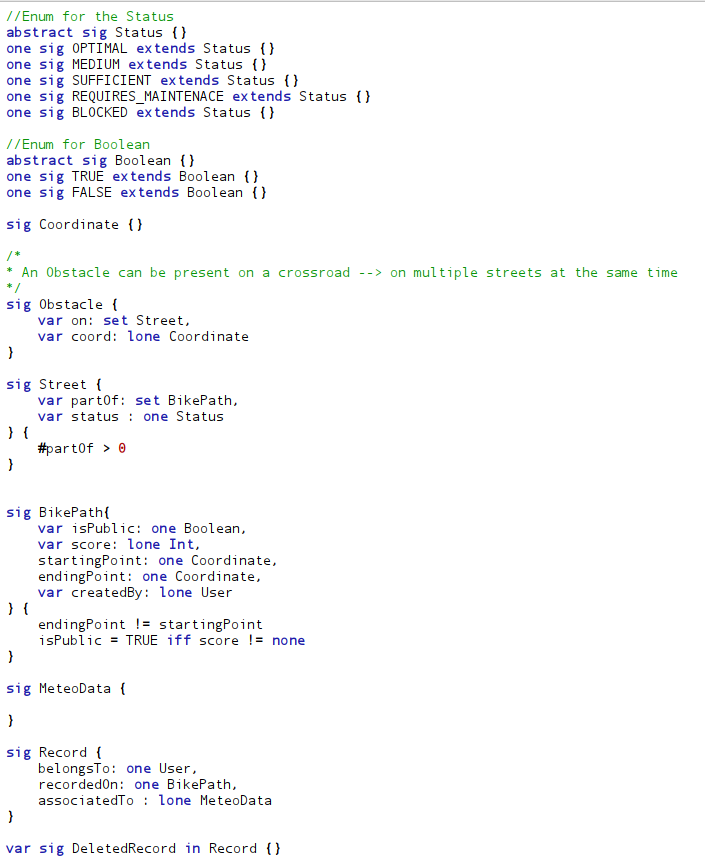
\includegraphics[width=1.0\linewidth]{images/Model_1st_section.png}
% \end{figure}
% \begin{figure}[t]
%     \centering
%     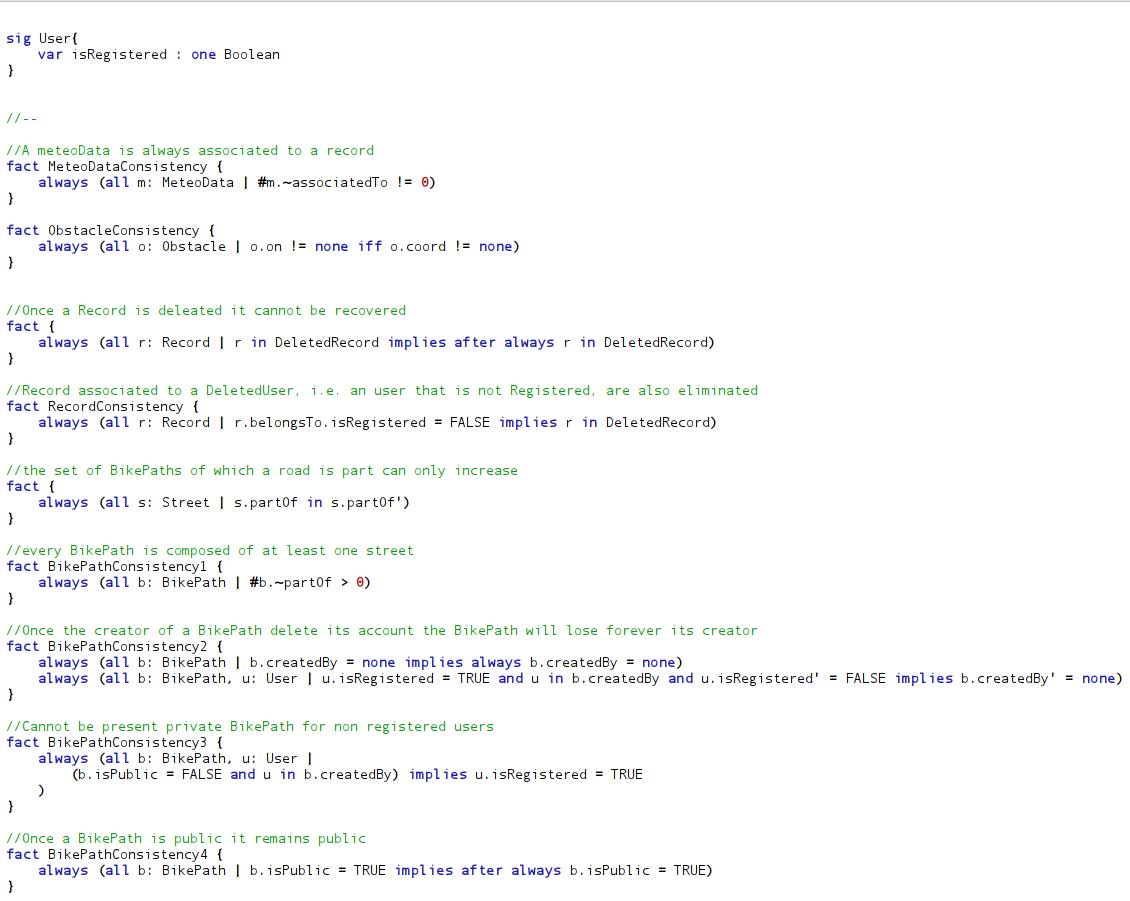
\includegraphics[width=1.0\linewidth]{images/Model_2nd_section.png}
% \end{figure}

\begin{minted}[
    linenos=true,         % Show line numbers
    framesep=2mm,         % Spacing between frame and code
    fontsize=\small,      % Font size
    style=default,        % Code highlighting theme (try default, colourful, or monokai)
    breaklines=true,      % Allow long lines to wrap
    tabsize=4,        
    obeytabs=true,    % Tells minted to process the tab as indentation
    showspaces=false, 
    frame=lines
]{alloy}
//Enum for the Status
abstract sig Status {}
one sig OPTIMAL extends Status {}
one sig MEDIUM extends Status {}
one sig SUFFICIENT extends Status {}
one sig REQUIRES_MAINTENANCE extends Status {}
one sig BLOCKED extends Status {}

//Enum for Boolean
abstract sig Boolean {}
one sig TRUE extends Boolean {}
one sig FALSE extends Boolean {}

sig Coordinate {} 
 
/*
* An Obstacle can be present on a crossroad --> on multiple streets at the same time
*/
sig Obstacle { 
	var on: set Street,
	var coord: lone Coordinate
} 

sig Street {
	var partOf: set BikePath,
	var status : one Status
} {
	#partOf > 0
}


sig BikePath{
	var isPublic: one Boolean,
	var score: lone Int,
	startingPoint: one Coordinate,
	endingPoint: one Coordinate,
	var createdBy: lone User
} {
	endingPoint != startingPoint
	isPublic = TRUE iff score != none
}

sig MeteoData {
	
}

sig Record {
	belongsTo: one User,
	recordedOn: one BikePath,
	associatedTo : lone MeteoData
}

var sig DeletedRecord in Record {}


sig User{
	var isRegistered : one Boolean
} 


//--

//A meteoData is always associated to a record
fact MeteoDataConsistency {
	always (all m: MeteoData | #m.~associatedTo != 0)
}

fact ObstacleConsistency {
	always (all o: Obstacle | o.on != none iff o.coord != none)
}


//Once a Record is deleted it cannot be restored
fact {
	always (all r: Record | r in DeletedRecord implies after always r in DeletedRecord)
}

//Records associated to a DeletedUser, i.e. an user that is not Registered, are also eliminated
fact RecordConsistency {
	always (all r: Record | r.belongsTo.isRegistered = FALSE implies r in DeletedRecord)
}

//The set of BikePaths of which a road is a part of, can only increase 
fact {
	always (all s: Street | s.partOf in s.partOf')
}

//Every BikePath is composed of at least one street
fact BikePathConsistency1 {
	always (all b: BikePath | #b.~partOf > 0)
}

//Once the creator of a BikePath deletes their account the BikePath will lose forever its creator
fact BikePathConsistency2 {
	always (all b: BikePath | b.createdBy = none implies always b.createdBy = none)
	always (all b: BikePath, u: User | u.isRegistered = TRUE and u in b.createdBy and u.isRegistered' = FALSE implies b.createdBy' = none)
}

//A private BikePath cannot be present for unregistered users
fact BikePathConsistency3 {
    always (all b: BikePath, u: User |
        (b.isPublic = FALSE and u in b.createdBy) implies u.isRegistered = TRUE
    )
}

//Once a BikePath is public it remains public
fact BikePathConsistency4 {
	always (all b: BikePath | b.isPublic = TRUE implies after always b.isPublic = TRUE)
}

//No unRegistered User can be the creator of a BikePath
fact BikePathConsistency5 {
	always (no u: User | some b: BikePath | u.isRegistered = FALSE and u in b.createdBy)
}

//A BikePath, if private, can only be in a Record associated to its owner
fact RecordConsistency {
	always (all r: Record, b: BikePath | b.isPublic = FALSE implies b.createdBy = r.belongsTo)
}



//A street with Obstacles can never be in OPTIMAL status
fact StreetConsistency {
	always (all s: Street | #s.~on > 0 implies s.status != OPTIMAL)
}

//The score changes olnly when:
//The state of a street that compose the path change
//The path is published
fact ScoreChange {
	always (all s: Street, b: BikePath |
			b in s.partOf and s.status = s.status' and b.isPublic = b.isPublic'implies b.score = b.score')
}
\end{minted}
\label{lst:fs_minted}

\noindent Let us argue some of the choices:
\begin{itemize}
    \item Once a 'BikePath' is created, it will remain forever public because it can be used by other users to make their own record. Deleting a 'BikePath' would mean destroying the recorded session of all users that used it.
    \item The 'Obstacle' indicates a generic type of obstacle and not a specific one. An obstacle is present in the physical universe only when it has coordinates and a street associated to it.
    \item Since a Street exists into the system only when someone uses it to create a 'BikePath', the set of 'BikePaths' of which a road is part can only increase.
    \item A 'MeteoData' can only exist within the system if associated to a Record.
\end{itemize}

\vspace{1cm}
\noindent Now let us show some scenarios where an obstacle appears on a certain street and then gets removed.

\begin{minted}[
    linenos=true,         % Show line numbers
    framesep=2mm,         % Spacing between frame and code
    fontsize=\small,      % Font size
    style=default,        % Code highlighting theme (try default, colourful, or monokai)
    breaklines=true,      % Allow long lines to wrap
    tabsize=4,        
    obeytabs=true,    % Tells minted to process the tab as indentation
    showspaces=false, 
    frame=lines
]{alloy}
pred firstScenario {
	some o: Obstacle, s: Street | {
		s not in o.on and after {
			s in o.on and after {
				removeObstacle[o]
			}
		}
	}
}
run firstScenario for 3 but 1 Street, 1 BikePath, 1 Obstacle, 0 Record
\end{minted}
\label{lst:fs_minted2}

% \begin{figure}[H]
%     \centering
%     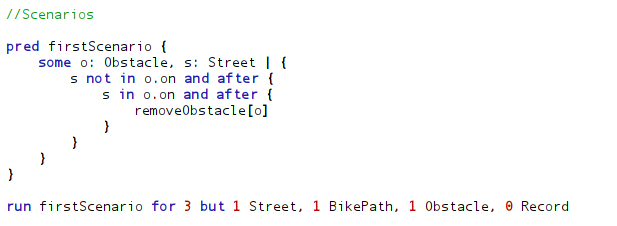
\includegraphics[width=1.0\linewidth]{images/First_Scenario_Definition.png}
% \end{figure}

% \begin{figure}[H]
%     \centering
%     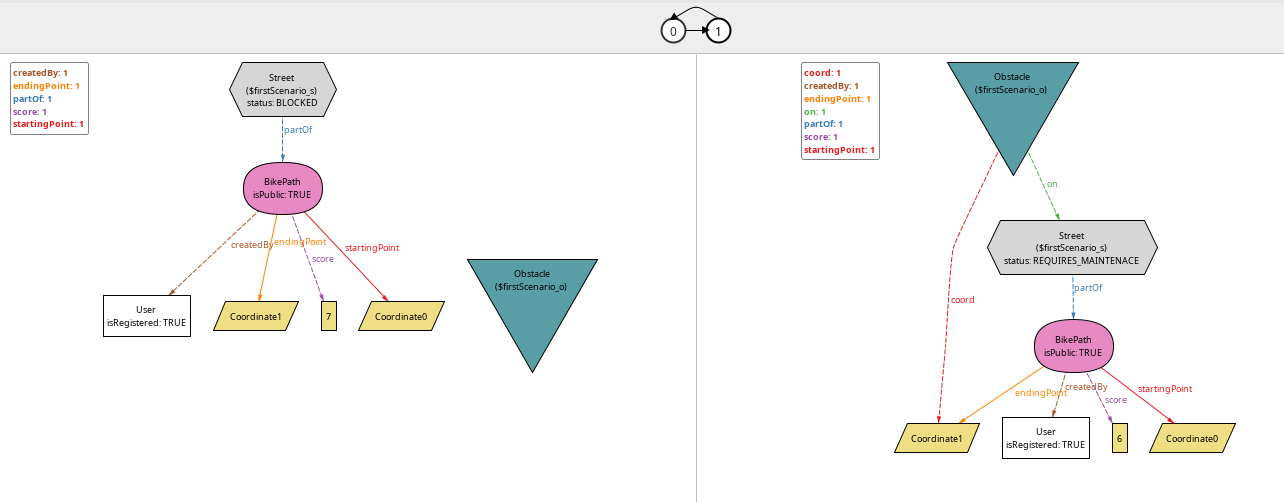
\includegraphics[width=1.0\linewidth]{images/First_Scenario_Universe.png}
% \end{figure}

\noindent\makebox[\textwidth][c]{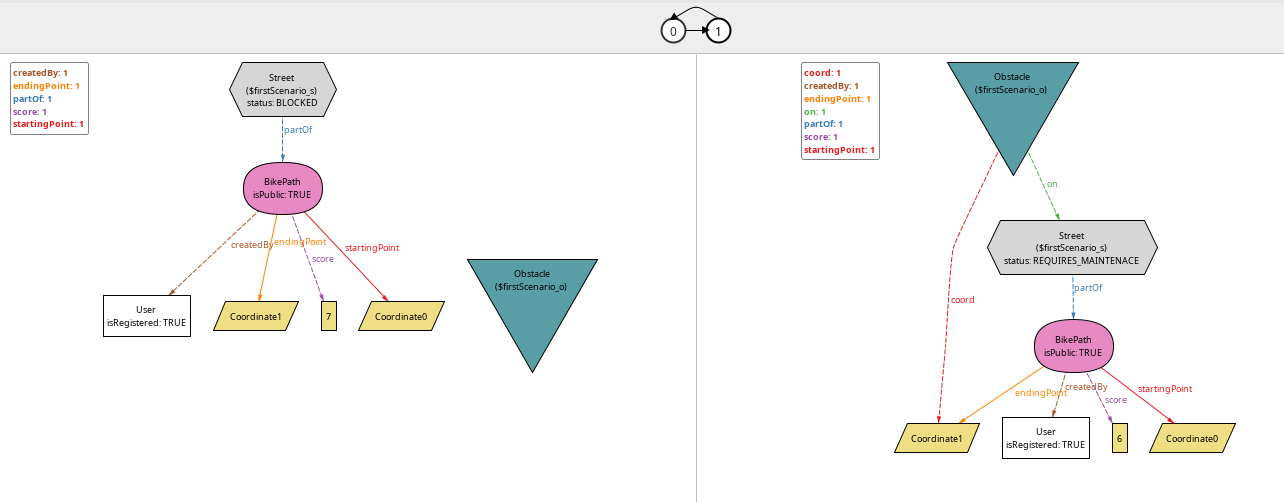
\includegraphics[width=1.3\textwidth]{images/First_Scenario_Universe.png}}

\bigskip
\noindent We can observe the followings: 
the model allows that a street can be BLOCKED also when there are no obstacles. This is perfectly acceptable because the streets may be closed for other reasons. Also, the presence of an obstacle does not necessarily mean that the street gets blocked: the obstacle may not affect the road's status to a point that makes it unusable.

% \noindent The following scenario shows a situation where a user publishes a private 'BikePath'.
% \begin{figure}[H]
%     \centering
%     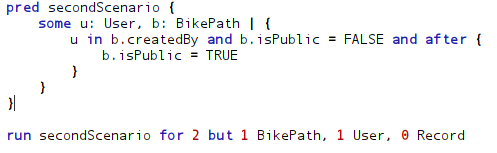
\includegraphics[width=1.0\linewidth]{images/Secondo_Scenario_Definition.png}
% \end{figure}
\begin{minted}[
    linenos=true,         % Show line numbers
    framesep=2mm,         % Spacing between frame and code
    fontsize=\small,      % Font size
    style=default,        % Code highlighting theme (try default, colourful, or monokai)
    breaklines=true,      % Allow long lines to wrap
    tabsize=4,        
    obeytabs=true,    % Tells minted to process the tab as indentation
    showspaces=false, 
    frame=lines
]{alloy}
pred secondScenario {
	some u: User, b: BikePath | {
		u in b.createdBy and b.isPublic = FALSE and after {
			b.isPublic = TRUE
		}
	}
}
run secondScenario for 2 but 1 BikePath, 1 User, 0 Record
\end{minted}
\label{lst:fs_minted3}

\vspace{0.5cm}
\noindent\makebox[\textwidth][c]{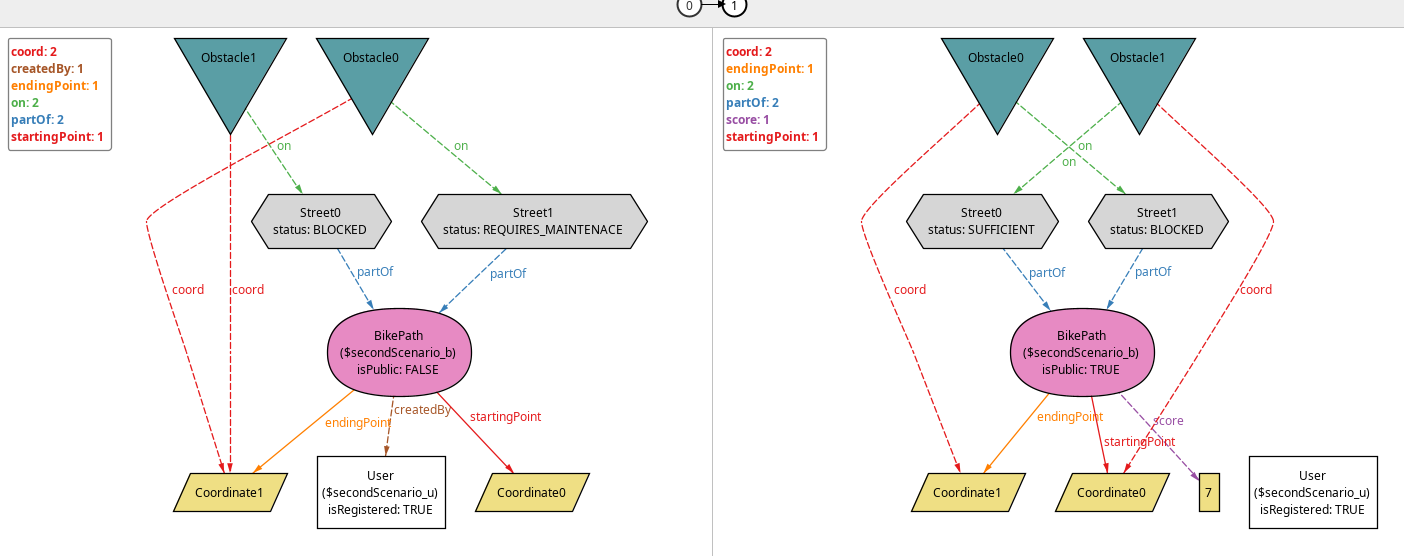
\includegraphics[width=1.3\textwidth]{images/Second_Scenario_Universe.png}}

\vspace{1cm}
\noindent We can observe that the 'BikePath' is correctly updated, i.e. it gets a score. 

\vspace{0.5cm}

\noindent We can also observe that a 'BikePath' can lose its creator. What happens will be
explained in the fourth scenario.

\vspace{0.5cm}

\noindent Let us now look at a scenario where a User deletes their account, let us observe how their record changes:

% \begin{figure}[H]
%     \centering
%     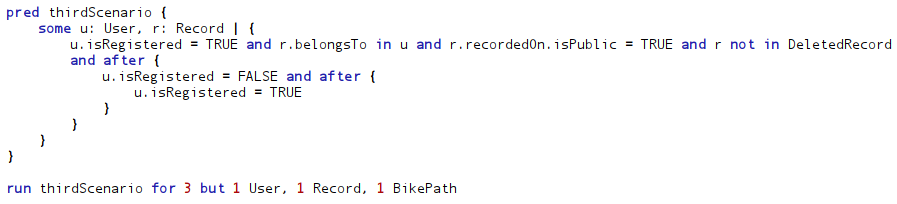
\includegraphics[width=1.0\linewidth]{images/ThirdScenario_Definition.png}
% \end{figure}

\begin{minted}[
    linenos=true,         % Show line numbers
    framesep=2mm,         % Spacing between frame and code
    fontsize=\small,      % Font size
    style=default,        % Code highlighting theme (try default, colourful, or monokai)
    breaklines=true,      % Allow long lines to wrap
    tabsize=4,        
    obeytabs=true,    % Tells minted to process the tab as indentation
    showspaces=false, 
    frame=lines
]{alloy}
pred thirdScenario {
	some u: User, r: Record | {
		u.isRegistered = TRUE and r.belongsTo in u and r.recordedOn.isPublic = TRUE and r not in DeletedRecord 
		and after {
			u.isRegistered = FALSE and after {
				u.isRegistered = TRUE
			}
		} 
	}
}
run thirdScenario for 3 but 1 User, 1 Record, 1 BikePath
\end{minted}
\label{lst:fs_minted4}

\vspace{0.5cm}
\noindent\makebox[\textwidth][c]{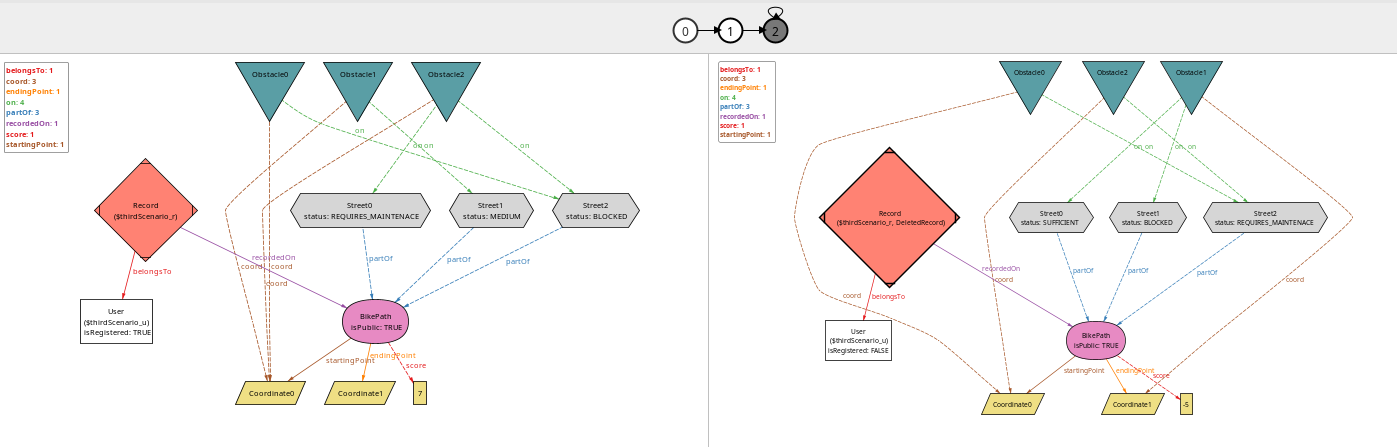
\includegraphics[width=1.3\textwidth]{images/ThirdScenario_Universe.png}}

\noindent The Record is correctly deleted. We can now observe that if the User creates a new Account the Record does not get restored:

\vspace{0.5cm}
\noindent\makebox[\textwidth][c]{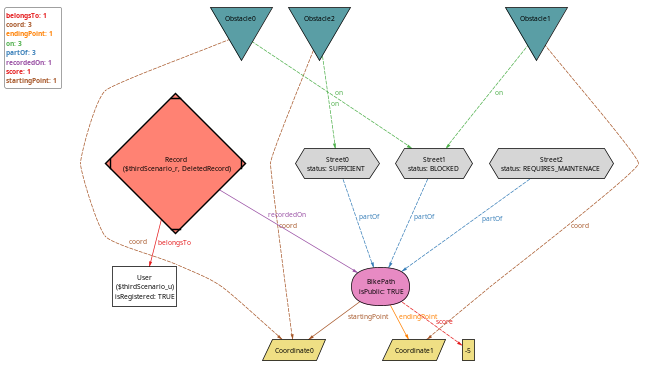
\includegraphics[width=1.0\textwidth]{images/ThirdScenario_Universe_p2.png}}

% \noindent The following scenario expands the situation briefly shown in the Second Scenario:
% \begin{figure}[H]
%     \centering
%     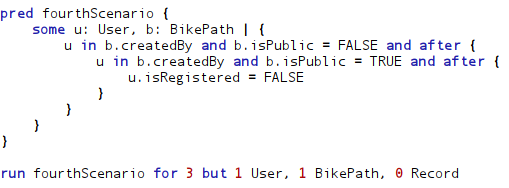
\includegraphics[width=1.0\linewidth]{images/FourthScenario_Definition.png}
% \end{figure}

\begin{minted}[
    linenos=true,         % Show line numbers
    framesep=2mm,         % Spacing between frame and code
    fontsize=\small,      % Font size
    style=default,        % Code highlighting theme (try default, colourful, or monokai)
    breaklines=true,      % Allow long lines to wrap
    tabsize=4,        
    obeytabs=true,    % Tells minted to process the tab as indentation
    showspaces=false, 
    frame=lines
]{alloy}
pred fourthScenario {
	some u: User, b: BikePath | {
		u in b.createdBy and b.isPublic = FALSE and after {
			u in b.createdBy and b.isPublic = TRUE and after {
				u.isRegistered = FALSE
			}
		}
	}
}
run fourthScenario for 3 but 1 User, 1 BikePath, 0 Record
\end{minted}
\label{lst:fs_minted5}

\begin{figure}[H]
    \centering
    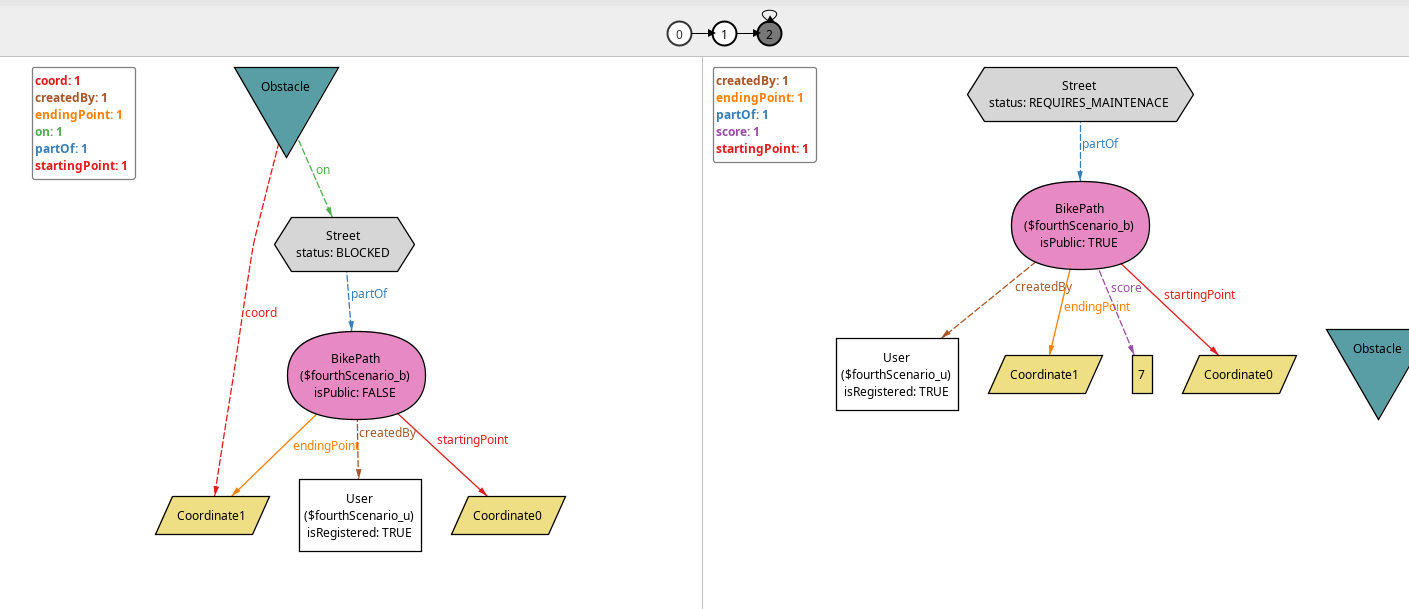
\includegraphics[width=1.0\linewidth]{images/Fourth_Scenario_Universe.png}
\end{figure}
\begin{figure}[H]
    \centering
    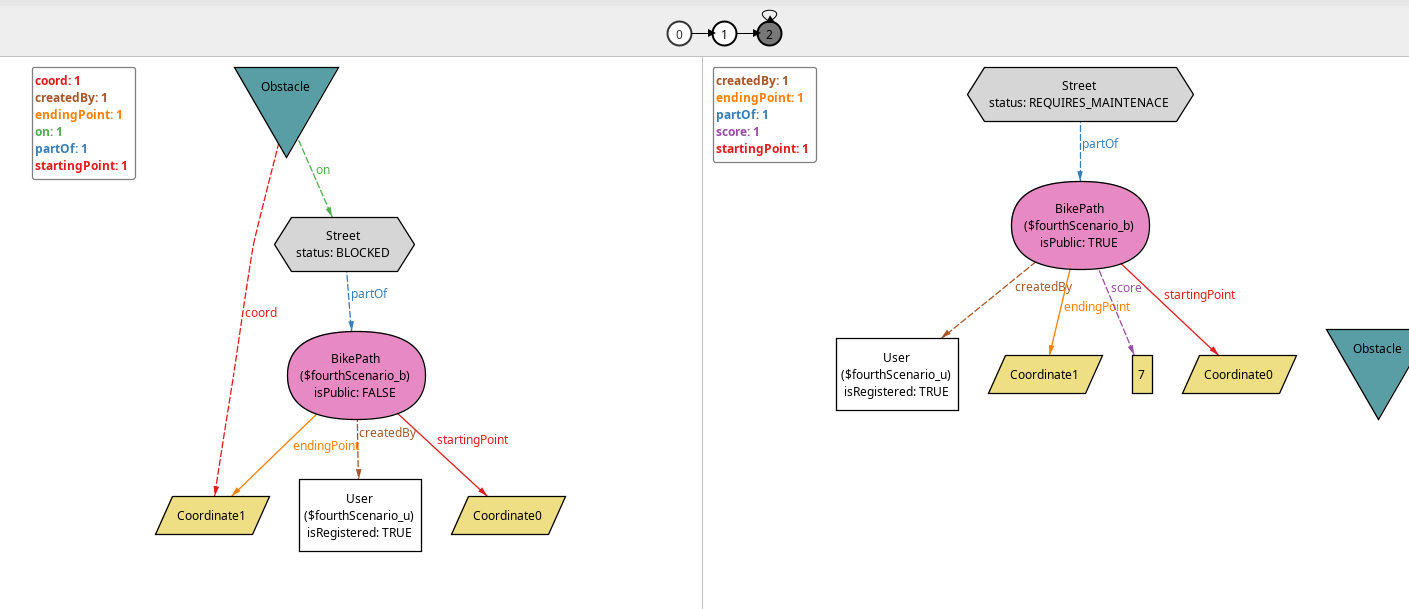
\includegraphics[width=1.0\linewidth]{images/FourthScenario_Universe_p2.png}
\end{figure}

\noindent We observe the following: for a registered User it is obviously possible to create and Publish a 'BikePath'. If the user decides to delete their account, the public 'BikePath' remains available and only loses its reference to the user that created it.

\bigskip

\noindent The following scenario shows how this particular situation is allowed in the model: 

% \begin{figure}[H]
%     \centering
%     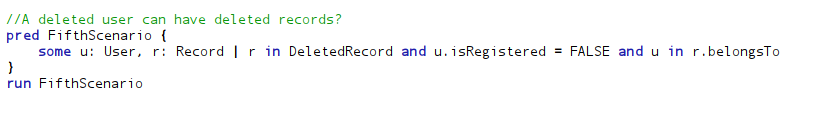
\includegraphics[width=1.0\linewidth]{images/FifthScenario_Definition.png}
% \end{figure}

\begin{minted}[
    linenos=true,         % Show line numbers
    framesep=2mm,         % Spacing between frame and code
    fontsize=\small,      % Font size
    style=default,        % Code highlighting theme (try default, colourful, or monokai)
    breaklines=true,      % Allow long lines to wrap
    tabsize=4,        
    obeytabs=true,    % Tells minted to process the tab as indentation
    showspaces=false, 
    frame=lines
]{alloy}
pred FifthScenario {
	some u: User, r: Record | r in DeletedRecord and u.isRegistered = FALSE and u in r.belongsTo
}
run fifthScenario
\end{minted}
\label{lst:fs_minted6}

% \begin{figure}[H]
%     \centering
%     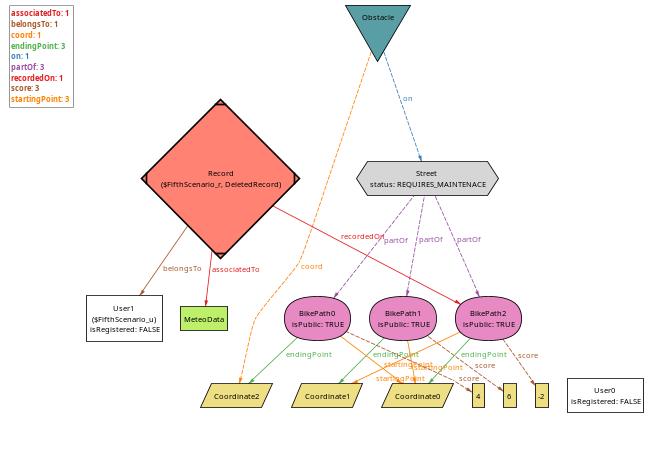
\includegraphics[width=1.0\linewidth]{images/FifthScenario_Universe.png}
% \end{figure}

\noindent\makebox[\textwidth][c]{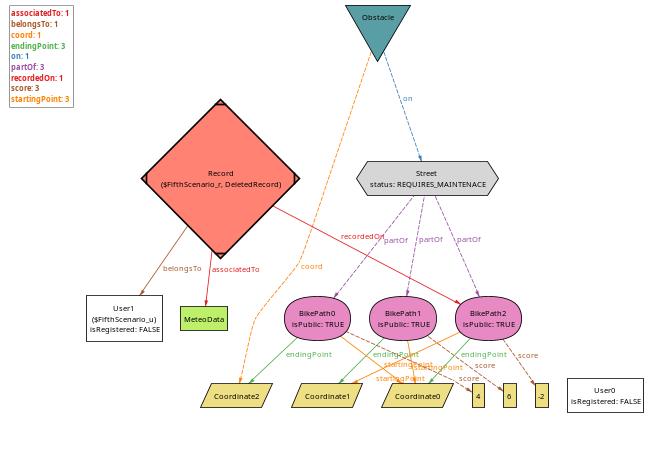
\includegraphics[width=1.0\textwidth]{images/FifthScenario_Universe.png}}

\bigskip

\noindent A Deleted Record can belong to a Deleted User. 
So far we have seen that a Deleted Record can belong to an unregistered User and a Registered User. We will prove that a non-deleted record cannot belong to a non-registered user in one the following assertions: 

% \begin{figure}[H]
%     \centering
%     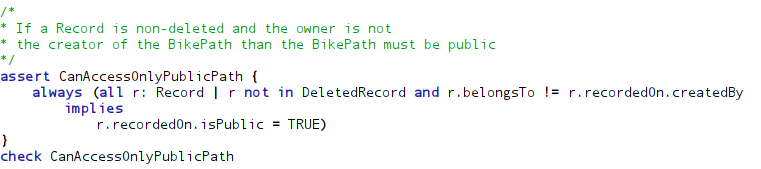
\includegraphics[width=1.0\linewidth]{images/FirstAssertionDefinition.png}
% \end{figure}

\begin{minted}[
    linenos=true,         % Show line numbers
    framesep=2mm,         % Spacing between frame and code
    fontsize=\small,      % Font size
    style=default,        % Code highlighting theme (try default, colourful, or monokai)
    breaklines=true,      % Allow long lines to wrap
    tabsize=4,        
    obeytabs=true,    % Tells minted to process the tab as indentation
    showspaces=false, 
    frame=lines
]{alloy}
/* If a Record is non-deleted and the owner is not 
* the creator of the BikePath, then the BikePath must be public
*/
assert CanAccessOnlyPublicPath {
    always (all r: Record | r not in DeletedRecord and r.belongsTo != r.recordedOn.createdBy
        implies
			r.recordedOn.isPublic = TRUE)
}
check CanAccessOnlyPublicPath
\end{minted}
\label{lst:fs_minted7}

\begin{figure}[H]
    \centering
    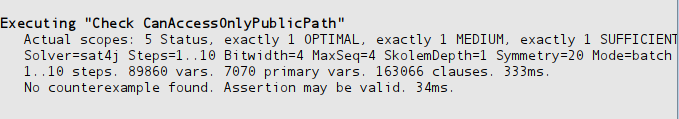
\includegraphics[width=1.0\linewidth]{images/FirstAssertionOutput.png}
\end{figure}

\bigskip

% \begin{figure}[H]
%     \centering
%     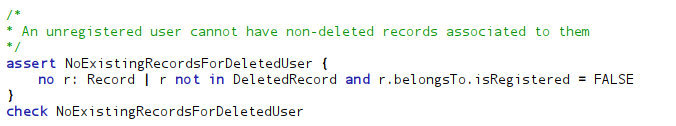
\includegraphics[width=1.0\linewidth]{images/SecondAssertionDefinition.png}
% \end{figure}

\begin{minted}[
    linenos=true,         % Show line numbers
    framesep=2mm,         % Spacing between frame and code
    fontsize=\small,      % Font size
    style=default,        % Code highlighting theme (try default, colourful, or monokai)
    breaklines=true,      % Allow long lines to wrap
    tabsize=4,        
    obeytabs=true,    % Tells minted to process the tab as indentation
    showspaces=false, 
    frame=lines
]{alloy}
/* An unregistered user cannot have non-deleted records associated to them
*/
assert NoExistingRecordsForDeletedUser {
	no r: Record | r not in DeletedRecord and r.belongsTo.isRegistered = FALSE
}
check NoExistingRecordsForDeletedUser
\end{minted}
\label{lst:fs_minted8}

\noindent\makebox[\textwidth][c]{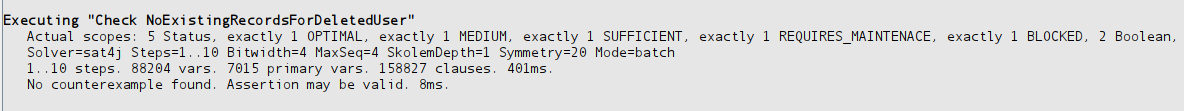
\includegraphics[width=1.3\textwidth]{images/SecondAssertionOutput.png}}

\newpage
\section{EFFORT SPENT}
The following table shows the approximate amount of hours that each group member spent on each chapter of this document. Please note that is calculation is only approximate, as each section still required active collaboration from all group members.
\begin{table}[h]
    \centering
    % \caption{Effort Spent (Hours)}
    \label{tab:effort}
    \begin{tabular}{|l|c|c|c|c|}
        \hline
        \textbf{Group Member} & \textbf{Chapter 1} & \textbf{Chapter 2} & \textbf{Chapter 3} & \textbf{Chapter 4} \\
        \hline
        A. Rubino & 6 & 1 & 1 & 25 \\
        \hline
        E. Uvinsi & 6 & 1 & 25 & 1 \\
        \hline
        I. Vinciguerra & 8 & 20 & 6 & 1 \\
        \hline
        \textbf{TOT} & \textbf{20} & \textbf{22} & \textbf{32} & \textbf{27} \\
        \hline
    \end{tabular}
\end{table}

\section{REFERENCES}
\begin{enumerate}
    \item \textbf{Project documents}:
        \begin{itemize}
            \item Specification document for the 2025/26 RASD project for the Software Engineering II course.
            \item Slides on the WeBeep page of the Software Engineering II course.
        \end{itemize}
    \item \textbf{Standards and regulations}:
        \begin{itemize}
            \item GDPR (General Data Protection Regulation).
        \end{itemize}
    \item \textbf{External service provider documentation/APIs}:
        \begin{itemize}
            \item Documentation or specifications for the MSP.
            \item Any specific API documentation or licensing terms mentioned for third-party software, libraries, or commercial mapping APIs.
        \end{itemize}
    \item \textbf{Technical specification documentation} for the following tools/protocols/formats:
        \begin{itemize}
            \item Alloy
            \item Standard geospatial data formats
            \item TLS 1.3
            \item JSON
        \end{itemize}
\end{enumerate}

\end{document}
